\documentclass{article}
\usepackage[utf8]{inputenc}
\usepackage{xcolor}
\usepackage[top=3cm,bottom=3cm,left=3.2cm,right=3.2cm,headsep=10pt,letterpaper]{geometry}

\usepackage{biblatex}                                    
\addbibresource{bibliography.bib}
\usepackage{graphicx}
\usepackage{siunitx}

\usepackage[acronym,nomain]{glossaries}                                  

\newacronym{lmc}{LMC}{Large Magellanic Cloud}
\newacronym{snr}{SNR}{Supernova Remnant}
\newacronym{pwn}{PWN}{Pulsar Wind Nebula}
\newacronym{pwne}{PWNe}{Pulsar Wind Nebulae}
\newacronym{vhe}{VHE}{Very High Energy}
\newacronym{he}{HE}{High Energy}
\newacronym{cta}{CTA}{Cherenkov Telescope Array}
\newacronym{sfh}{SFH}{Stellar Formation History}
\newacronym{ms}{MS}{Magellanic System}
\newacronym{smc}{SMC}{Small Magellanic Cloud}
\newacronym{mw}{MW}{Milky Way}
\newacronym{ism}{ISM}{Interstellar Medium}
\newacronym{ulrigs}{ULRIGs}{Ultraluminous Infrarred Galaxies}
\newacronym{ic}{IC}{Inverse Compton}
\newacronym{cmb}{CMB}{Cosmic Microwave Background}
\newacronym{sm}{SM}{Standard Model}
\newacronym{dm}{DM}{Dark Matter}
\newacronym{wimp}{WIMP}{Weak Interacting Massive Particle}
\newacronym{gc}{GC}{Galactic Center}
\newacronym{iact}{IACT}{Imaging Atmospheric Cherenkov Telescope}
\newacronym{ksp}{KSP}{Key Science Projects}
\newacronym{fov}{FoV}{Field of View}
\newacronym{roi}{ROI}{Region of Interest}
\newacronym{irf}{IRF}{Instrument Response Function}
\newacronym{cl}{CL}{Confidence Level}

\newcommand{\sigv}{\langle \sigma v \rangle}
\newcommand{\mdm}{m_{\chi}}
\newcommand{\MB}[1]{{\color{orange}[{\bf Mab:} #1]}}
\newcommand{\FI}[1]{{\color{blue}[{\bf FI:} #1]}}
\newcommand{\EK}[1]{{\color{magenta}[{\bf EK:} #1]}}
\newcommand{\MJB}[1]{{\color{purple}[{\bf MB:} #1]}}


\title{Characterization of the Large Magellanic Cloud at TeV energies with the CTA}
\author{M. I. Bernardos, F. Iocco, P. Martin}

\date{}

\begin{document}

\maketitle
\begin{abstract}
    The Large Magellanic Cloud is a nearby galaxy, spatially resolved, with a very interesting population of gamma ray sources. Previous observations of the LMC by Fermi LAT and H.E.S.S., have revealed the presence of a diffuse gamma ray emission and several sources with rare features, such as the most luminous Pulsar Wind Nebula N157B, the most luminous gamma ray binary LMC P3, the most luminous X-ray Supernova Remnant N132D and the rare non-thermal superbubble 30DorC. Also, its high dark matter mass $\sim 10^{10}\odot$ makes it a natural target for indirect dark matter searches. 
    In this paper we explore the potential of the upcoming Cherenkov Telescope Array on its future observations of the Large Magellanic Cloud. We have performed simulations of the emission model of the LMC and calculated detection prospects on the known sources and possible new ones. 
    We set limits on the possible models for the diffuse gamma ray emission of the LMC and we have performed sensitivity studies for the detection of a Dark Matter annihilation signal, using different \gls{dm} profiles, annihilation channels and \gls{dm} masses.
    We have concluded that the CTA will be able to explore the diffuse emission of the LMC with a sensitivity without precedents being able to detect it at more than 5$\sigma$ in the most optimistic models. We calculate that it will be able to detect more than $~20$ new gamma ray sources (Pulsar Wind Nebulae) and it will set strong upper limits on dark matter models. 
    
\end{abstract}
\section{Introduction}
The \gls{lmc} is one of the closest satellite galaxies of the \gls{mw}, at a distance of $\sim$ 50 kpc \cite{2013LMCdistance1}. Thanks to its proximity, large volume and orientation angle ($\sim$ 30º \cite{2004StructureandOrientationLMC}), it is observed as an extended object of about 10º diameter in the sky, which has allowed the study of its structure and individual components in great detail. Observations of the \gls{lmc} in the whole electromagnetic spectrum have revealed the presence of a big number of extreme objects such as pulsars \cite{2013RadioPulsarsLMC} \cite{2016LMCFermiLAT}, \glspl{snr} \cite{2015MultiwavelengthLMCsnr} \cite{2012XMM1987} \cite{2016SNRinXrayLMC},  \gls{pwne} \cite{2015HESSTeVLMC} \cite{2016LMCFermiLAT} \cite{2003PWNeintheLMC} \cite{2008PWNeXrayLMC} and gamma--ray binaries \cite{2017HESSLMCP3}. Many of these objects are known to be cosmic-ray accelerators and therefore plausible gamma--ray emitters. Gamma-ray emission up to TeV energies from several sources within the \gls{lmc} has already been detected by the current generation gamma--ray experiments \textit{Fermi}-LAT and H.E.S.S. and it is expected that many more objects will be discovered by the future \gls{cta}.\\
The remarkable interest of the \gls{lmc} for gamma--ray astrophysics relies on its high star formation activity, which implies a high supernova rate and thus the large population of gamma--ray sources,
and the possibility it offers to study the relation between star formation and cosmic-ray production and propagation.\\
Cosmic rays are an important component of \gls{ism} in galaxies, with energy densities comparable to that of magnetic fields. The origin and propagation of cosmic-rays is still a field of study as well as their role in galaxy evolution. It is very likely that they have a significant effect in star formation, acting as an extrinsic feedback source. The basic idea is that, even the energy injection rate of cosmic rays is negligible compared to other by-products of star formation such as photons, winds and supernova shocks, they interact with the \gls{ism} and exchange a significant amount of momentum. Studies on Starburst galaxies luminosities \cite{2008SocratesCRandSF} have established that it is possible that cosmic-ray winds are produced in high star formation rate regions, perturbing the hydrostatic balance and truncating star formation. On the other hand, infrarred observations of \gls{ulrigs} suggest that cosmic-rays are able to heat gas in molecular clouds and are their main agent of temperature regulation and ionization, fundamentally altering the initial conditions for star formation \cite{2010PapadopoulosCRinSF}.\\
While \gls{lmc} evolution is closely related to the \gls{mw} and the rest of the local group, the observations of very young globular clusters in the \gls{lmc} suggests that its \gls{sfh} is fundamentally different to that of the \gls{mw} \gls{sfh}. In fact, the \gls{lmc} is currently in a star formation epoch with a rate of $\sim$ 0.2 $M_{\odot}$ which was reignited 4-5 Gyrs ago after a dramatic event affecting the \gls{ms} (composed by the \gls{lmc} and the \gls{smc}, not covered in this text) \cite{2009SFHofLMC}. The \gls{lmc} is classified as an irregular galaxy, the most common type in the universe. In general, irregular galaxies are simpler, less dusty and with lower metallicity than spiral galaxies (like the \gls{mw}). Because they are less evolved, they present higher gas content and lower abundance of heavy elements \cite{2013InfrarredLMC}. All these features affecting the characteristics of the \gls{ism} are fundamental for the study of their effects in the production and propagation of cosmic-rays, and allow to use the \gls{lmc} as an alternative probe to the \gls{mw} for cosmic-ray studies.\\
Characterizing the cosmic-ray origin and propagation throughout the \gls{ism} is not an easy task, because they as charged particles are deflected by magnetic field, making it impossible to reconstruct their trajectories and thus, pointing back to their origin form Earth. The best way to study the cosmic-ray physics in the galaxies is through the diffuse emission from radio to gamma--rays that they produce when interacting with other particles in the \gls{ism} and the radiation and magnetic fields. The leptonic component of this emission, produced by cosmic-ray electrons, can be probed by radio, X-ray and gamma--ray observations. The radio diffuse emission come from synchrotron emission of cosmic-ray electrons injected by supernova remnants. They can also suffer \gls{ic} scattering with photons of the interstellar radiation field or the cosmic microwave background, producing emission from X-ray to gamma--rays \cite{2008ICgammaray}. The hadronic component of diffuse cosmic-ray emission is produced (mainly) by cosmic-ray protons inelastic collisions with the \gls{ism} particles, which can produce pions resulting in a high energy gamma--ray emission coming from pion decay \cite{1963Pimesonsproducegammarays}. Therefore, gamma--rays are a fundamental probe for cosmic-ray production and propagation, because hadrons make up the 90\% of the cosmic-ray composition.\\ 
A galaxy like the \gls{lmc}, externally viewed and nearly face on offers an unique opportunity for studying the diffuse emission of cosmic-rays, in comparison with the \gls{mw} which has the problem of line-of-sight confusion of sources. \textit{Fermi}-LAT observations of the \gls{lmc} revealed a diffuse gamma--ray emission little correlated with the large scale distribution of the gas column density of the galaxy \cite{2010FermiLATLMC11months}. This correlation would be observed if cosmic-rays could freely diffuse in the \gls{ism} as it is observed in the \gls{mw}. Instead, it appears to be much more correlated with tracers of massive star forming regions such as the 30 Doradus region \cite{2012CRinLMC30Doradus}.\\
Beyond the extraordinary opportunities for cosmic-ray physics, the \gls{lmc} offers also the possibility to help solving the fundamental problem of \gls{dm}. There are many probes that suggest that the universe is composed of something more than the visible matter: From the Fritz Zwicky measurements on the velocity dispersion in the Coma galaxy cluster \cite{Zwicky} and the rotation curves of high-luminosity spiral galaxies obtained by Vera Rubin \cite{1978Rubin}, to the measurements of the \gls{cmb} by Planck \cite{2014Planck}, all of them point to the existence of a non-baryonic type of matter which only interacts gravitationally with \gls{sm} particles. The \gls{lmc} has a mass of the order of $10^9$ M$_{\odot}$ enclosed in 8.9 kpc and more than a half is due to a dark halo \cite{2002LMCkinematics}. Study of the rotational curves of the \gls{lmc} revealed that also it must contain a dark compact bulge with an anomalously high mass-to-luminosity ratio as large as $\sim 20-50$ \cite{1999LMCbulge} compared of that of the calculated for the \gls{mw} $\sim$ 7 M/L \cite{2013MWbulge}. With these characteristics, \gls{lmc} would be the most \gls{dm} massive object after the \gls{gc} offering an alternative source for indirect searches of \gls{dm} signal.\\
Among all the theories trying to explain the nature of \gls{dm}, the \gls{wimp} theory is one of the most popular, explaining \gls{dm} as a particle which can suffer annihilation or decay into \gls{dm} particles. Different channels of annihilation would produce a certain spectrum of gamma--rays \cite{2011cirelli} which could be detected as an excess over the gamma--ray flux produced by baryonic backgrounds. Following this scheme, \textit{Fermi}-LAT used five years of data to search for a \gls{dm} annihilation signal in gamma--rays and placed competitive bounds on the annihilation cross section as a function of the dark matter particle mass and annihilation channel \cite{2010FermiLATLMC11months}.\\
The future of ground based $\gamma$-ray astronomy is in hands of the \gls{cta} currently in construction. \gls{cta} will be a gamma--ray observatory without precedents, as the result of combined efforts of scientists from all over the astroparticle physics community. It will have two locations, one observatory in the northern hemisphere in the island of La Palma, Spain, and the other in the south, in the Atacama desert, Chile. It will account for three types of telescopes (Large, Medium and Small size) which will allow to do full sky observations, with a sensitivity one order of magnitude better than the current generation of \gls{iact} observatories, with an energy range from 20 GeV to 300 TeV and a resolution up to 2 arcsecs. The \gls{lmc} Survey is one of the \gls{ksp} of \gls{cta} \cite{2019SciencewithCTA}, with more than 300h of dedicated observations and many scientific objectives: population studies of \glspl{snr} and \gls{pwne}, transport of cosmic-rays and searches of \gls{dm}. 
In this paper we perform a characterization of the \gls{lmc} in the energy range of \gls{cta}, in order to cast predictions on the possible results of the \gls{lmc} survey. Our methodology is to build an emission model of the \gls{lmc} and use a dedicated \gls{cta} software to perform simulations of the survey data products. We use a maximum likelihood approach to calculate the detection significance of the different sources of gamma--rays in the \gls{lmc}, as well as the possibilities for setting a realistic model of the diffuse cosmic-ray emission. In the same way, we calculate sensitivity curves for the detection of a possible \gls{dm} annihilation signal. The structure of the paper is as follows:
In section \ref{sec:model} we describe the emission model we use for the \gls{lmc}. Section \ref{sec:simana} is dedicated to details on simulation and analysis methods for \gls{cta} observations. In section \ref{sec:res} results on significance for detection of diffuse emission and point sources in the LMC are presented. In section \ref{sec:dminlmc} we describe the models of a possible \gls{dm} emission from the \gls{lmc} and we calculate sensitivity curves for \gls{cta} detection of such signal. In section \ref{sec:systematics} possible systematics mainly related to the instruments are discussed. Finally, section \ref{sec:conclusions} is dedicated to conclusions.

\section{Emission Model} \label{sec:model}
     
    \subsection{Diffuse emission} \label{sec:diffusemodel}
    Description of the model(s) used for Pion Decay and IC.
    \subsection{Point Sources}
    
    Observations in gamma--rays of the \gls{lmc} have provided a very interesting catalog of point-like sources of different nature, which have revealed very interesting features. For this work, we use the \gls{lmc} data collected by \textit{Fermi}-LAT \cite{2010FermiLATLMC11months} \cite{2016LMCFermiLAT} and H.E.S.S. \cite{2012HESSLMC} \cite{2015HESSTeVLMC} \cite{2017HESSLMCP3} to build the emission models of the sources we have decided to include in this study. A description of the different point sources and their emission model is given in this section.
    
    \subsubsection{Pulsar Wind Nebula N157B}
    
    Gamma-ray emission from the direction of the \gls{pwn} N 157B associated to the pulsar  PSR J053-6910 has been measured both by \textit{Fermi}-LAT in the \gls{he} range ($\sim 10 \sigma$) and by H.E.S.S. in the \gls{vhe} range ($33 \sigma$). This is the first and only \gls{pwn} ever detected outside the \gls{lmc} in gamma rays \cite{2012HESSN157B}. \gls{pwne} are the result from  a supernova explosion, where a fast-rotating, highly-magnetized central pulsar powers a nebula of ultrarelativistic particles with its spin-down energy, i.e. the loss rate of rotational energy. The well known Crab \gls{pwn} is an object of this kind, which seems to present large similarities with N157B. The central pulsar of this system, PSR J053-6910 was first discovered in X-ray energies and seems to be the most powerful pulsar known, with a spin-down power of $\Delta E = 4.9 \cdot 10^{34} $ erg s$^{-1}$ \cite{1998PulsarN157B}. The TeV gamma--ray emission of this kind of objects is directly connected to their spin-down power and has its origin in the \gls{ic} scattering of lower energy photons by relativistic electrons (and positrons). Besides its extremely high power, the emission from N157B can be detected despite its large distance ($\sim 48 kpc$ \cite{2006N157Bdistance}) because it is embedded in the strong infrared photon-fields from nearby sources of the superbubble formed by the stellar association LH99 \cite{}, which serve as additional targets for the \gls{ic} scattering.
    To model this source, we follow the results from \cite{2015HESSTeVLMC}, where the multiwavelength data (X-rays from Chandra \cite{2001ChandraN157B} and gamma--rays from \textit{Fermi}-LAT and H.E.S.S.) can only be exp2006N157Bsuperbubblelained with a leptonic \gls{ic} model where the highest possible magnetic field should be 45$\mu$ G. The  spectral model adopted for this source is shown in figure \ref{fig:psourcesspec}. 
    
    \subsubsection{Supernova Remnant N132D}
    
    Both \textit{Fermi}-LAT and H.E.S.S. have detected gamma--ray emission with strong evidences to belong to the \gls{snr} N 132D, a very bright thermal X-ray remnant. It is the brightest remnant of the \gls{lmc} and belongs to a rare type of oxygen-rich remnants which show optical emission from pure heavy-element ejecta, similar to the \gls{mw} \gls{snr} Cas A \cite{2007N132D}. The origin of this \gls{snr}, deduced by its chemical composition, is the core-collapse supernova of a massive progenitor star of $> 35 M_{\odot}$ \cite{2007N132D}. The origin of the gamma--ray emission yields on the interaction of the supernova shock with the cloud of dense material ejected by the progenitor star during its lifetime. The flux detected by H.E.S.S. \cite{2015HESSTeVLMC}, with a gamma--ray luminosity in the 1-10 TeV band of $0.9 \pm 0.2 \times 10^{35}(d/50kpc)^2$ erg/s, allow to contemplate the possibility of two possible origins of the radiation: In the hadronic scenario the flux of gamma--rays is produced by the decay of neutral-pions, which would imply a remarkably high fraction of energy injected to cosmic rays by the supernova explosion, or a gas density higher than the one expected from X-ray observations. Either possibility is plausible given the observations in the optical and infrarred bands, which reveals a structure produced by the interaction of the remnant with shocked interstellar gas \cite{2006shockn132D}. In the leptonic scenario, gamma rays are produced by \gls{ic} scattering of low energy-photons. This model could be supported by the high synchrotron radio emission in radio and X-rays, however, it would require a lower magnetic field than the one inferred from radio observations ($20 \mu G$ vs. $40\mu G$). The fluxes and spectral index measured by \textit{Fermi}-LAT in \cite{2016LMCFermiLAT} seem to rule out this model.\\
    For this work, we use the hadronic model shown in figure \ref{fig:n132D} based on H.E.S.S. measurements. 
    
    \subsubsection{Superbubble 30 Dor C}
    
    The Superbubble 30 Dor C, detected by H.E.S.S. in the \gls{vhe} range, is a radiation emitting shell which stands out in X-rays, being the largest X-ray synchroton shell known (with a radius of 47pc) \cite{200430dorcxrays}, and also emits radio and optical radiation \cite{1985SNRsintheLMC30dorc}. Its origin seems to be related to the stellar winds and supernovae of the stellar association LH 90 \cite{198430dorLH90}. Both a leptonic and hadronic scenario could explain the gamma--ray flux detected by H.E.S.S. from this source as discussed in \cite{2015HESSTeVLMC}. The two models are shown in figure \ref{fig:psourcesspec}. For this work we tested the both models, knowing that \gls{cta} observations from 100 GeV will be very likely able to set which is the most probable model, thanks to the slope differences up to 1 TeV.
     
     \begin{figure}
        \centering  
        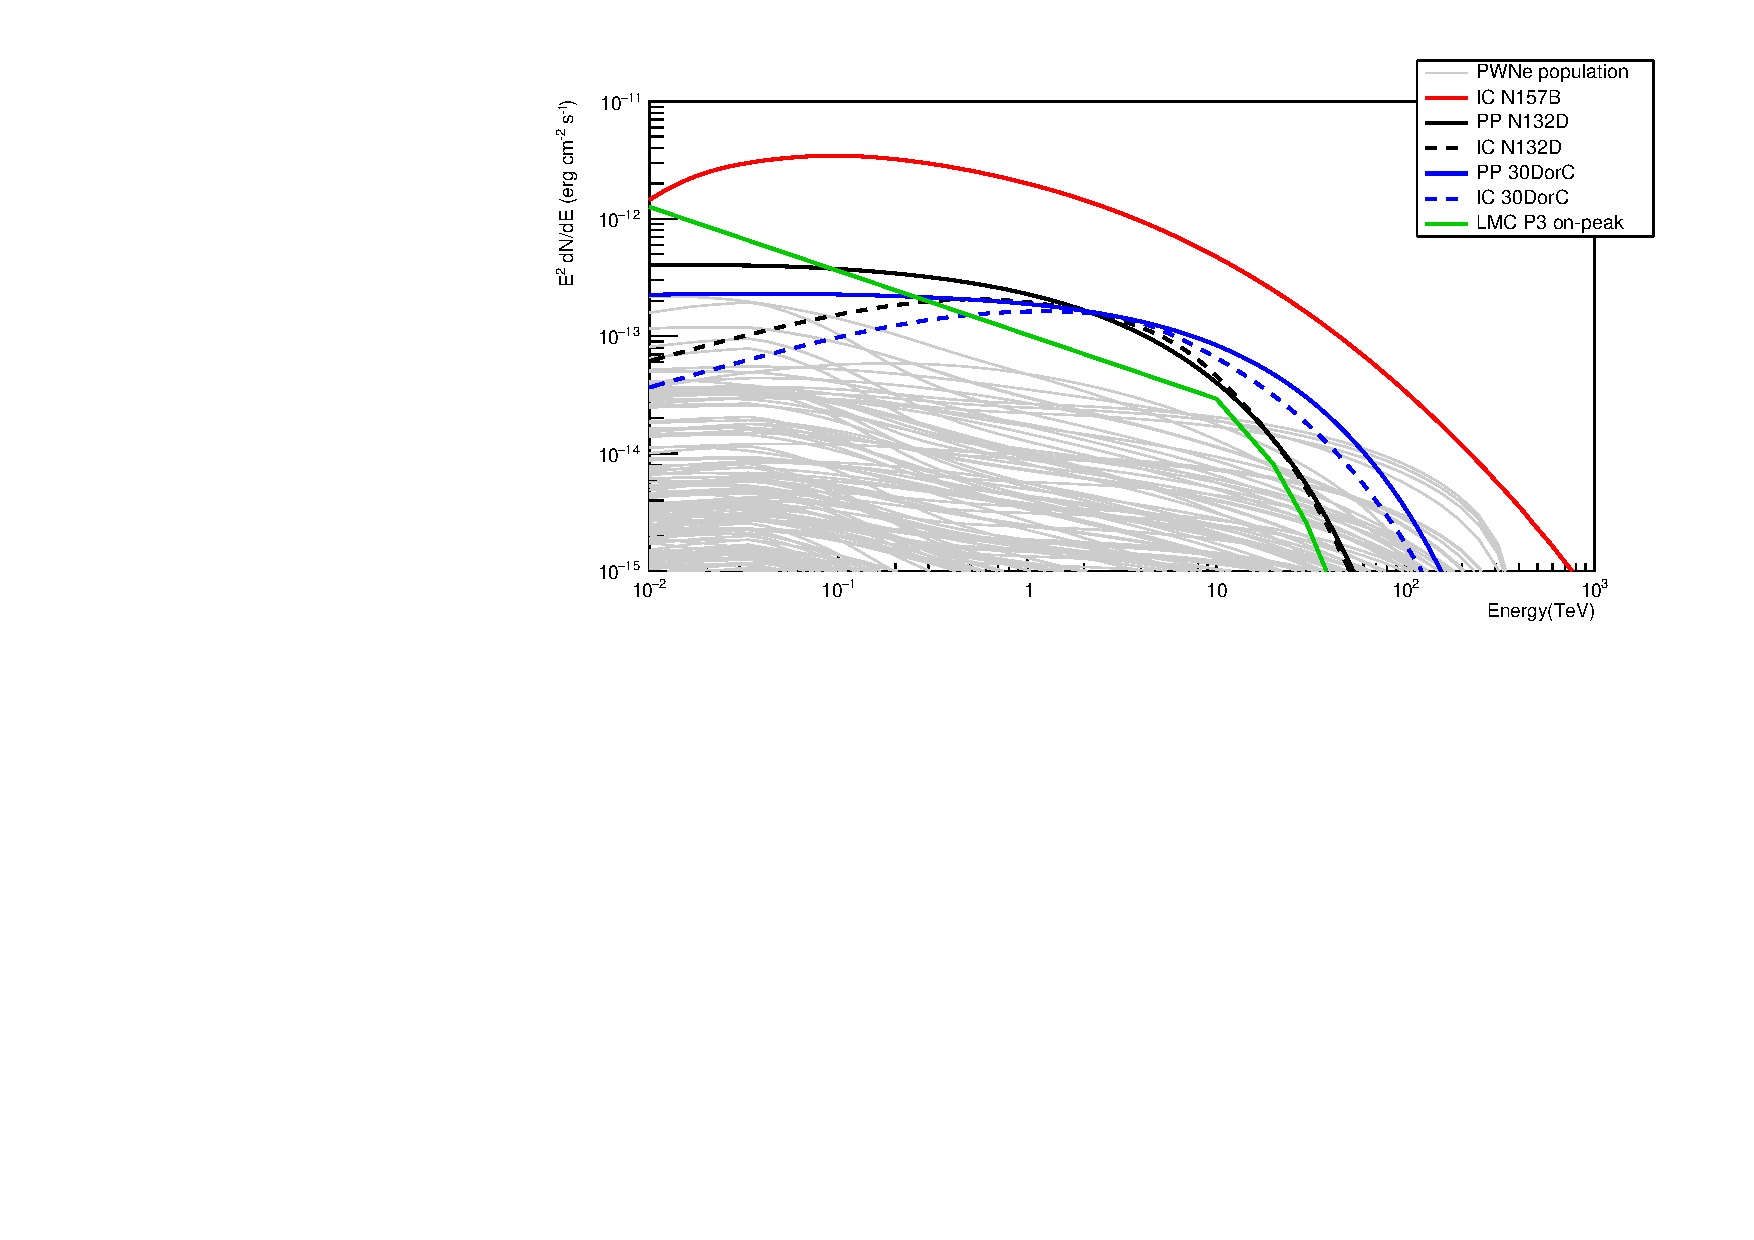
\includegraphics[width=\textwidth]{Pictures/pointsourcesspec.pdf}
        \caption{\label{fig:psourcesspec} Spectral energy distribution of the point sources in the \gls{lmc}. Spectra from N157B, N132D and 30DorC are extracted from \cite{2015HESSTeVLMC}. Spectrum of LMC P3 is a power-law with the spectral parameters of the on-peak orbital region from \cite{2017HESSLMCP3}, with an exponential cut-off at 10 TeV. Spectra from the \gls{pwne} population are derived following the baseline model described in section \ref{sec:pwnepop}}
    \end{figure}
     
    \subsubsection{Binary system LMC P3}
    This object was first detected by \textit{Fermi}-LAT at \gls{he} energies in \cite{2016LMCFermiLAT}, but was classified as an unidentified source in the environment of the HII regions NGC 2029/NGC2032. They measured a very soft power-law spectrum (index $\sim 2.8$) but dit not notice any variability down to a monthly basis.
    Later, emission from this object in the \gls{vhe} range was detected by H.E.S.S. \cite{2017HESSLMCP3}. They discovered a variability of 10.3 period, classifying the object as the first extragañactic gamma--ray binary system. The position of LMC P3 is consistent with a soft X-ray source, which variability of X-ray flux and radial velocity of Balmer absorption lines confirmed that it is very likely a binary system \cite{1981softXraysLMC}, \cite{2012xraybinaryP3}. From optical radial velocity measurements, it is derived that the system must be composed by a neutron star with an O5III star companion \cite{2016P3binary}. Gamma-ray binaries are believed to be a brief phase of the evolution of high-mass X-ray binaries, in which the gamma--ray emission dominates the electromagnetic output \cite{1989binaries}.\\
    The spectrum of LMC P3 (HESS J0536-675) was fitted by H.E.S.S. to a simple power law of the form $\frac{dN}{dE} = \Phi_{1TeV}\left( \frac{E}{1TeV}\right)^{-\Gamma}$ with an on-peak spectral index $\Gamma$ of 2.1, and an off-peak index of 2.4, where on-peak represents the orbit region where most of the gamma--ray radiation is emitted. The detection of the source only achieved enough statistical significance during the on-peak period.\\
    For simplicity in this work, we will assume the on-peak spectral parameters of the source without any temporal modulation ($\Gamma=2.1$, $\Phi_{1TeV} = 5 \cdot 10^{-13}cm^{-2}s^{-1}TeV^{-1}$). The justification is that the on-peak orbital phase lasts for $\sim 50$h, which is way below the total observation time assigned to the \gls{lmc} survey. A test on the possibility of detecting the off-peak emission with \gls{cta} is also carried in section[]. The spectrum of the on-peak power law is shown in picture \ref{fig:psourcesspec}.
     
    \subsection{PWNe population} \label{sec:pwnepop}
    Description of how we come up with the PWNe population in the LMC.


\section{Simulations and Analysis method} \label{sec:simana}

    \subsection{Region of Interest and Observational strategy}

As before mentioned, the  \gls{roi} of the \gls{lmc} extends about 10º in the sky. In order to reach this large \gls{fov}, \gls{cta} will adopt a novel survey mode, which is an observational technique never applied before by \glspl{iact}. It will consist on covering the full region by a series of slightly overlapping pointings with a \gls{fov} of $\sim 3º$ each. The total amount of hours assigned to the \gls{lmc} survey is 340h plus 150h more in case the \gls{snr} 1987A is detected. For this work, different pointing patterns have been tested in order to adopt the observational strategy which will maximize the significance of detection both for point sources and extended sources, for a total observation time of 340h. The final scheme consist on 7 pointings of $\sim 1.75 \times 10^5$s each, arranged in 3 rows with a 2-3-2 configuration centered in the coordinates RA=80.0º, dec=-69.0º with a separation of 2º between pointings, as shown in figure \ref{fig:pointings}. In this observation mode, all telescope types of \gls{cta} South are involved.

\begin{figure}
  \centering
  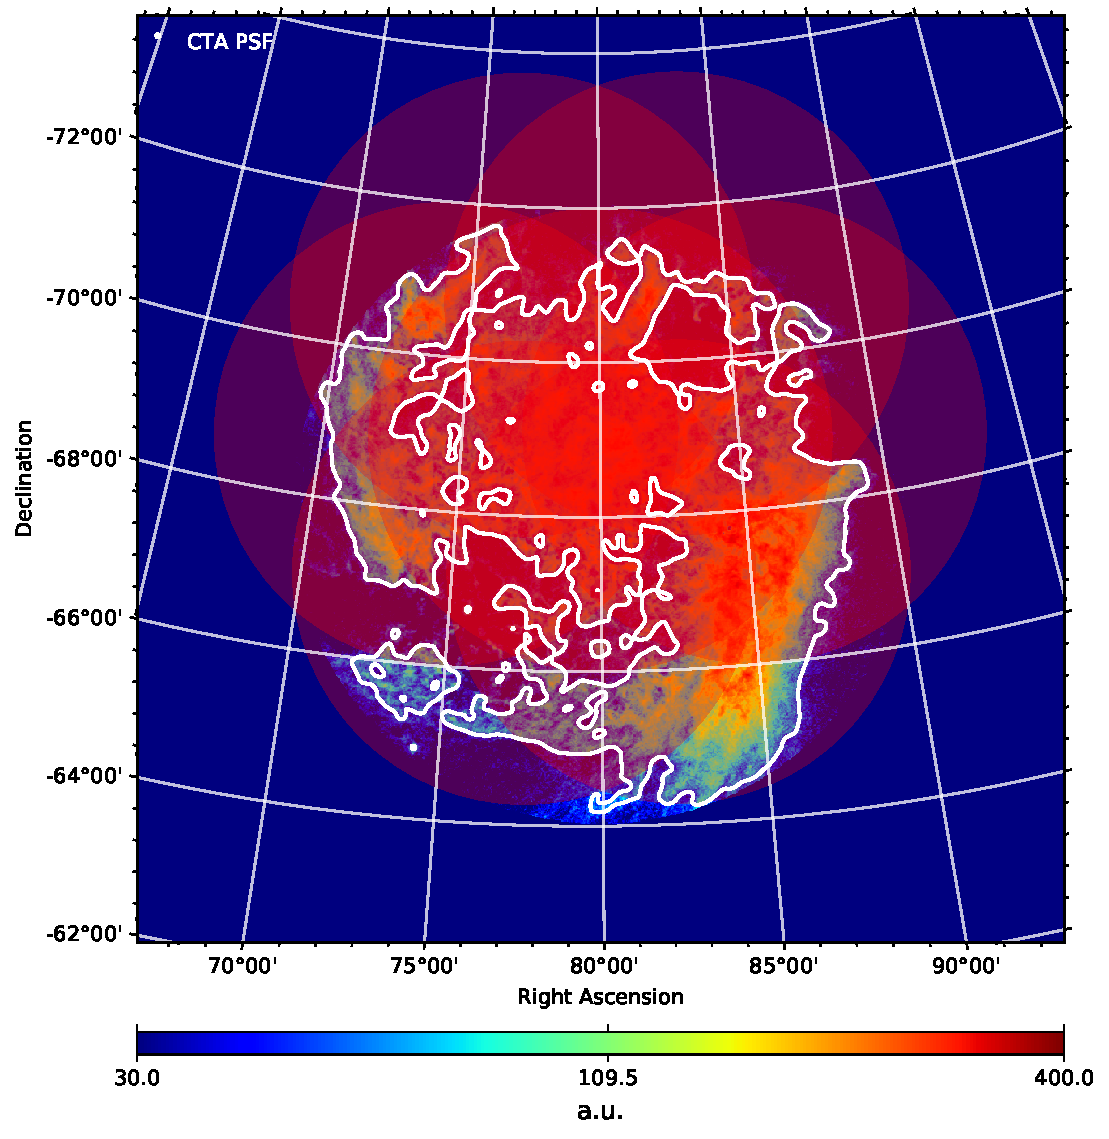
\includegraphics[width=0.7\textwidth]{Pictures/lmc_hi_cdensity_flipped_plot_1000GeV_1TeV.pdf}
  \caption{\label{fig:pointings} Skymap of the region of interest of the \gls{lmc}. The pointing pattern is overlapped in the shape of red circles.}
\end{figure}

\subsection{Simulation parameters}

To calculate the predicted number of counts from a certain emission model, the \gls{cta} collaboration provides a set of \glspl{irf} \cite{CTAPerformance} with information about the effective area and angular resolution of the instrument for several zenith angles. For this work we have used the \gls{irf} \textit{South\_z40\_50h} from the production \textit{prod3b-v2}. This \gls{irf} only accounts for the southern observatory and is optimized for zenith angles around 40º (\gls{lmc} will be seen at $\sim 46$º from the southern site) and 50h observations. \\
To perform the simulations of the predicted number of counts using the mentioned pointing pattern and \gls{irf} we use \textit{ctools} and \textit{gammalib} \cite{2016Actools}, a software framework for the analysis of astronomical $\gamma$-ray data, specifically designed for \gls{cta}. The tool \textit{ctobssim} uses a \gls{mc} generator to recreate event lists for observations. As input, it requires a full model of the \gls{roi}, including each individual source with a spatial and spectral component, and a model of the instrumental background accounting for cosmic-ray events misidentified as $\gamma$s.
Also, \textit{ctobssim} requires the \gls{irf} for the observation and the desired energy range must be specified. Each running of \textit{ctobssim} results in a realization of the model where the event list is generated with a random number generator. We have performed realizations of the full emission model of the \gls{lmc} with the pointing pattern described before, in the energy range from 0.05 TeV to 150 TeV. \textit{Ctobssim} is able to combine the different observations of the overlapping pointings, averaging the \glspl{irf} of each region. The resulting event lists are written into FITS files, one for each pointing, which can be combined afterwards for the analysis.\\
The tool \textit{ctmodel} uses the resulting event lists from \textit{ctobssim} and the emission model to calculate an averaged expected number of events. Instead of one realization of the model, it represents the expected number of counts that will be obtained by an infinitely large number of realizations. The result is a counts map, where the averaged number of counts is given for each spatial pixel and for each energy bin.

\subsection{Fitting method}

A binned likelihood analysis has been performed in this work, to fit the emission model to the simulated data. The event lists for the 7 pointings have been combined and then the data has been binned into $\sim$ 110 energy bins. The boundaries of the energy bins have been generated using the \textit{ctools} function \textit{csbins}, which inspects the variation in the effective area and background template of the \gls{irf} for the specific simulations, according to a threshold settled by the user. To ensure a sufficiently large number of energy bins (it is recommended to have at least 30 bins per decade), the threshold for the fractional change in effective area has been settled to 0.06, and to 0.16 for background rate. \\
The energy range chosen for the analysis is from 100 GeV to 100 TeV. The higher lower limit, compared to the full range of \gls{cta} (which can go down to 30 GeV) comes from the limitations of performance at high zenith angles, given that \gls{lmc} will be always observed at z > 40º.
For the combination of data the procedure for stacked analysis of \textit{ctools} has been followed, where the binned counts map of the data is produced using the function \textit{ctbin} and then the combined background model, the exposure cube and the point spread function cube are precomputed using the functions \textit{ctbkgcube}, \textit{ctexpcube} and \textit{ctpsfcube} respectively. The results are a series of mapcubes which will be used to calculate the maximum likelihood function.\\
A so-called \textit{Asimov} data set has been computed to produce the results presented in this chapter. The \textit{Asimov} data set \cite{2011Asimov} is a representative data set which, when fitted, will retrieve the true values of the model parameters. It can be computed with \textit{ctools} using the function \textit{ctmodel}, and allow to give mean results for significance and upper limits without needing a large number of realizations of the simulated data.\\
The mapcube of the Asimov dataset produced for this analysis is shown in picture \ref{fig:asimov} for the 0.975-1.04 TeV energy bin. 
\begin{figure}
  \centering
  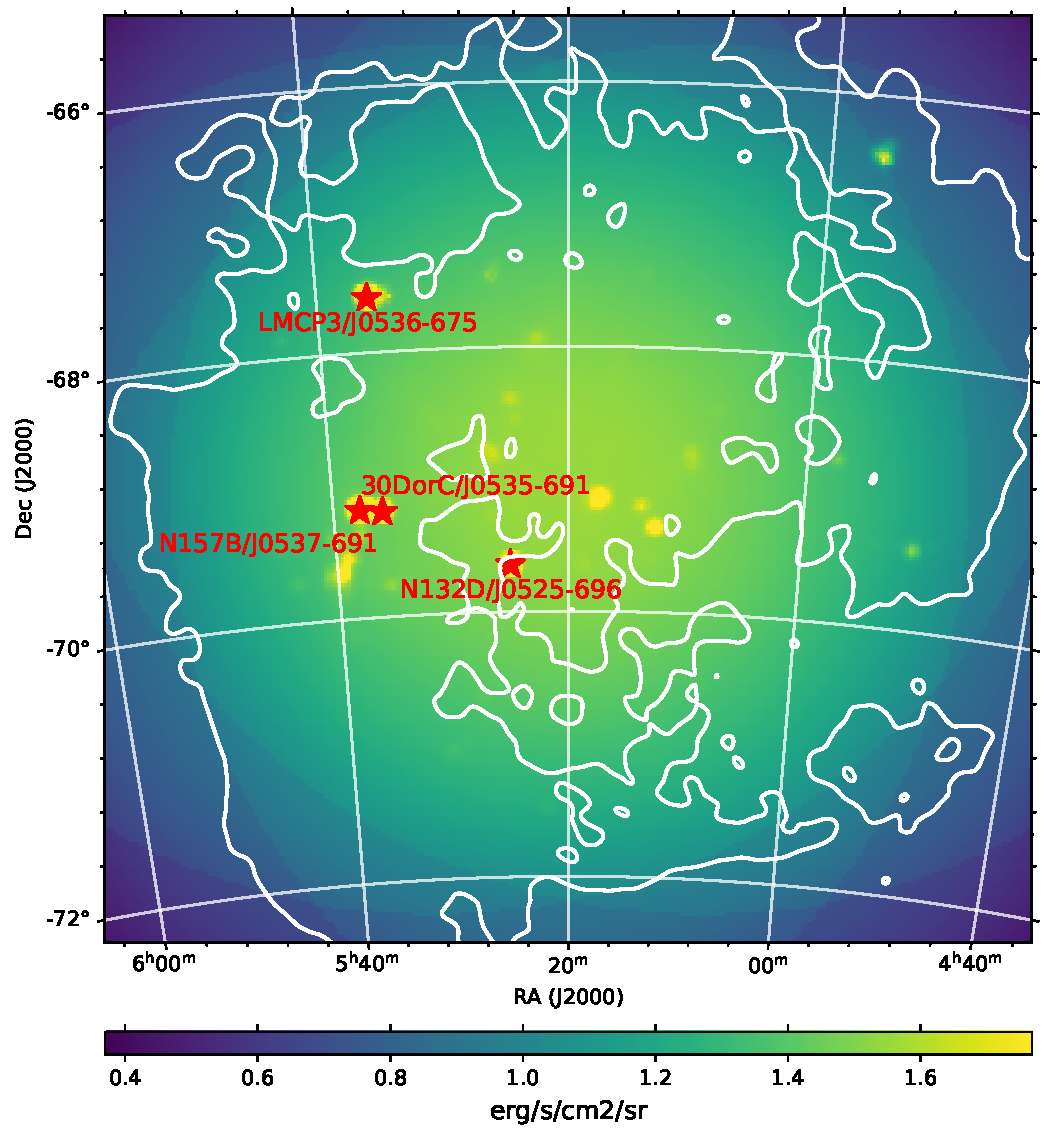
\includegraphics[width=0.6\textwidth]{Pictures/Asimov_0-975_1-04TeVmap.pdf}
  \caption{\label{fig:asimov} Asimov mapcube at the energy bin 0.975-1.04 TeV produced with the full emission model of the \gls{lmc} described in section \ref{sec:model}. The four point sources are marked with red stars.  }
\end{figure}
\subsubsection{3D Likelihood Analysis for $\gamma$-ray sources}
The likelihood analysis is based in the typical Poisson likelihood function:
\begin{equation}
  \mathcal{L}(\mu | n) = \prod_{i,j}\frac{\mu_{ij}^{n_{ij}}}{n_{ij}!}e^{-\mu_{ij}}
  \label{eq:likelihood}
\end{equation}

Where $n_{ij}$ represents the simulated counts and $\mu_{ij}$ the model prediction for each bin in energy(i) and space (j). The model $\mu_{ij}$ is the result of the combination of the models for each of the $\gamma$-ray sources described in section \ref{sec:model}. Each source accounts for a spectral model and a spatial model. For extended sources, both components are combined in one mapcube. In the likelihood fitting the only free parameter for each of these models is the normalization $A^{X}$, which determine the relative weight of component $X$. The only exception is the point source LMC P3, which spectral model is a power-law where the free parameters are the normalization and the spectral index. The shape of $\mu$ is:

\begin{equation}
  \mu_{ij}(A^{X}) = \sum_{X} A^{X} \mu^{X}_{ij} + A^{LMC P3}(E)^{-\Gamma}
\end{equation}

The maximum likelihood is calculated finding the normalization parameters $A^{X}$ which maximize equation \ref{eq:likelihood}.\\
The detection significance of a source is calculated in terms of the Test Statistics:

\begin{equation}
  TS = 2log \frac{\mathcal{L}(\mu(A^{X})|n)}{\mathcal{L}_{null}}
  \label{eq:ts}
\end{equation}

Where $\mathcal{L}(\mu(A^{X})|n)$ is the maximum likelihood function and $\mathcal{L}_{null}$ is the value of the likelihood function of the null hypothesis for the specific source (meaning $A^X$ = 0). With this definition, typically a source is considered to be detected when $TS>25$, equivalent to $5\sigma$.\\
The maximum likelihood analysis has been performed using the function \textit{ctlike} from \textit{ctools}. The inputs are the data mapcubes from the stacked analysis and the description of the emission model. For the likelihood fit the same emission model used for the simulations is given as input, meaning that the fitting results will represent the most optimistic case, where the model is perfectly describing the data. \textit{ctlike} calculates the best fit parameters ($A^X$, $\Gamma$) and the TS values for the requested sources (setting the variable tscalc=''1'').

\subsubsection{Upper limits calculation} \label{sec:ulimits}

For sources which have a flux too low to be detected ($TS < 25$) we calculate upper limits on the minimum flux needed for the source to be detected with \gls{cta}. We calculate this upper limits as the flux that leads to a decrease in the likelihood that corresponds to a certain \gls{cl}. Using the definition of TS from \ref{eq:ts}, according to Wilks' theorem \cite{wilks1938}, the TS function asymptotically approaches a $\chi^2$-distribution with one degree of freedom under the null hypothesis, therefore to get the flux that yields to the 95\% \gls{cl} upper limit, we must find the normalization parameter $A^X_{max} > A^{X}$ which corresponds to TS = 2.71.\\
This calculation is performed using the function \textit{ctulimit} from \textit{ctools}, which requires as input the mapcube of the simulated data and a model with all the sources, including the source for which the upper limit will be calculated. In this case, we use the model resulting from the maximum likelihood fit. The only free parameters must be the normalizations. The results from \textit{ctulimit} are the upper limit in the differential flux for a reference energy, the integrated upper flux limit for a specific energy range and the integrated upper energy flux limit for the same range.\\
We have used this method to set constraints on the \gls{dm} annihilation cross section $<\sigma v>$ as described in section \ref{sec:dminlmc}.
    
\section{Results}\label{sec:results}
        
\subsection{Point sources}

The results for the fitting of the four point sources tested in this work are given in table \ref{tab:fitsources}. The significance of detection of the sources is given in terms of the Test Statistics described in the previous section. For LMC P3 three cases have been tested: The case of a spectrum following a power-law with the on-peak parameters from \cite{2017HESSLMCP3}; the same power-law but with an exponential cut-off at 10 TeV; and a last case where no source has been simulated, but an upper limit on the flux for a source with the off-peak spectral index has been computed in the energy range 0.1-100 TeV. Also, energy flux upper limits for three energy ranges are shown in figure \ref{fig:sensiulimits}.\\
The point sources have been fitted in the full energy range to the same models used for simulation, where the only free parameter is the spectral normalization.
The results show that \gls{cta} will be able to detect with high significance all the known point sources in the \gls{lmc}, including the binary system \gls{lmc} during the on-peak orbital region, and will be able to test the flux of the off-peak region. 


\begin{table}
  \centering
  \resizebox{\textwidth}{!}{%
  \begin{tabular}{llllll}
    \hline
    Source name & RA(º) & Dec(º) & Normalization & TS & Significance($\sigma$) \\
     &  &  & $(0.1 - 100 TeV)$ &  &  \\
    \hline
    & & Point Sources & & & \\
    \hline
    N157B/HESS J0537-691 & 84.44 & -69.18 & $1\pm 0.005$ & 130951.51 & 361.9 \\
    N132D/HESS J0525-696 & 81.26 & -69.64 & $1\pm 0.019$ & 5370.19 & 73.3\\
    30DorC/HESS J0535-691 (PP) & 83.96 & -69.2 & $0.999 \pm 0.022$ & 4762.83 & 69.0 \\
    30DorC/HESS J0535-691 (IC) & 83.96 & -69.2 & $0.999 \pm 0.022$ & 3919.0 & 62.6 \\
    LMCP3/HESS J0536-675 & 84.0 & -67.59 & Prefactor: $4.99\pm0.05 \cdot 10^{-19}$ & 27353.83 & 165.4 \\
    (on-peak, cut-off 10 TeV) &  &  & $(cm^{-2}s^{-1}MeV^{-1})$ &  &  \\
    & &  & Index: $2.1 \pm 0.01 $ &  &  \\
    LMCP3/HESS J0536-675 & 84.0 & -67.59 & Prefactor: $4.99\pm0.05 \cdot 10^{-19}$ & 48021.95 & 219.14 \\
    (on-peak)&  &  & $(cm^{-2}s^{-1}MeV^{-1})$ &  &  \\
    & &  & Index: $2.1 \pm 0.006 $ &  &  \\
    LMCP3/HESS J0536-675 & 84.0 & -67.59 & Int. flux ulimit (99 \% CL): $1.23 \cdot 10^{-13}$ & - & - \\
    (off-peak)&  &  & $(cm^{-2}s^{-1})$ &  &  \\
    \hline
    & & Diffuse emission components & & & \\
    \hline
    LMC Pion-decay & - & - & $1\pm0.185$ & 29.06 & 5.39 \\
    LMC IC & - & - & Int. flux ulimit(99\% CL): $7.33 \cdot 10^{-12}$ & - & - \\
     &  &  & $(cm^{-2}s^{-1})$ &  &  \\
  \end{tabular}}
  \caption{Results of the fit for the point sources and diffuse components included in the emission model. For the first three sources, the normalization of the spectrum is the only free parameter to fit. For LMCP3, a power-law spectrum with exponential cut-off at 10 TeV has been fitted, accordingly with the results of \cite{2017HESSLMCP3}. For the off-peak region, the upper limit at 99\% \gls{cl} for the integrated flux has been calculated. From the diffuse components, only the hadronic emission could be detected at $TS>25$ therefore an upper limit has been computed for the leptonic \gls{ic} component. }
  \label{tab:fitsources}
\end{table}

\subsection{Population of PWNe}

For the fitting of the \gls{pwne} population, a mapcube including all the artificially computed candidates has been used for simulation. Then, each \gls{pwn} spectrum has been fitted individually, keeping all the rest of the \gls{pwne} and other model components fixed. The results show that 15 from the total of 189 simulated \gls{pwne} would be detected with $TS>25$, giving an estimation of the number of new \gls{pwne} that could be discovered by \gls{cta}. Also, 12 more \gls{pwne} were fitted giving a $TS>9$ ($3\sigma$ significance). 
It must be taken into account that this is a very optimistic result, giving that the true spectrum and position of each \gls{pwne} is being used for fitting. In reality, a totally blind search will be performed, scanning the full region in the search for excesses, and assuming a generic spectral shape. The results on the \gls{pwne} are shown in figure \ref{fig:pwnepopresults}, showing the fitted flux compared to the true flux, and the TS value vs. the true flux.

\begin{figure}
\centering
\minipage{0.5\textwidth}
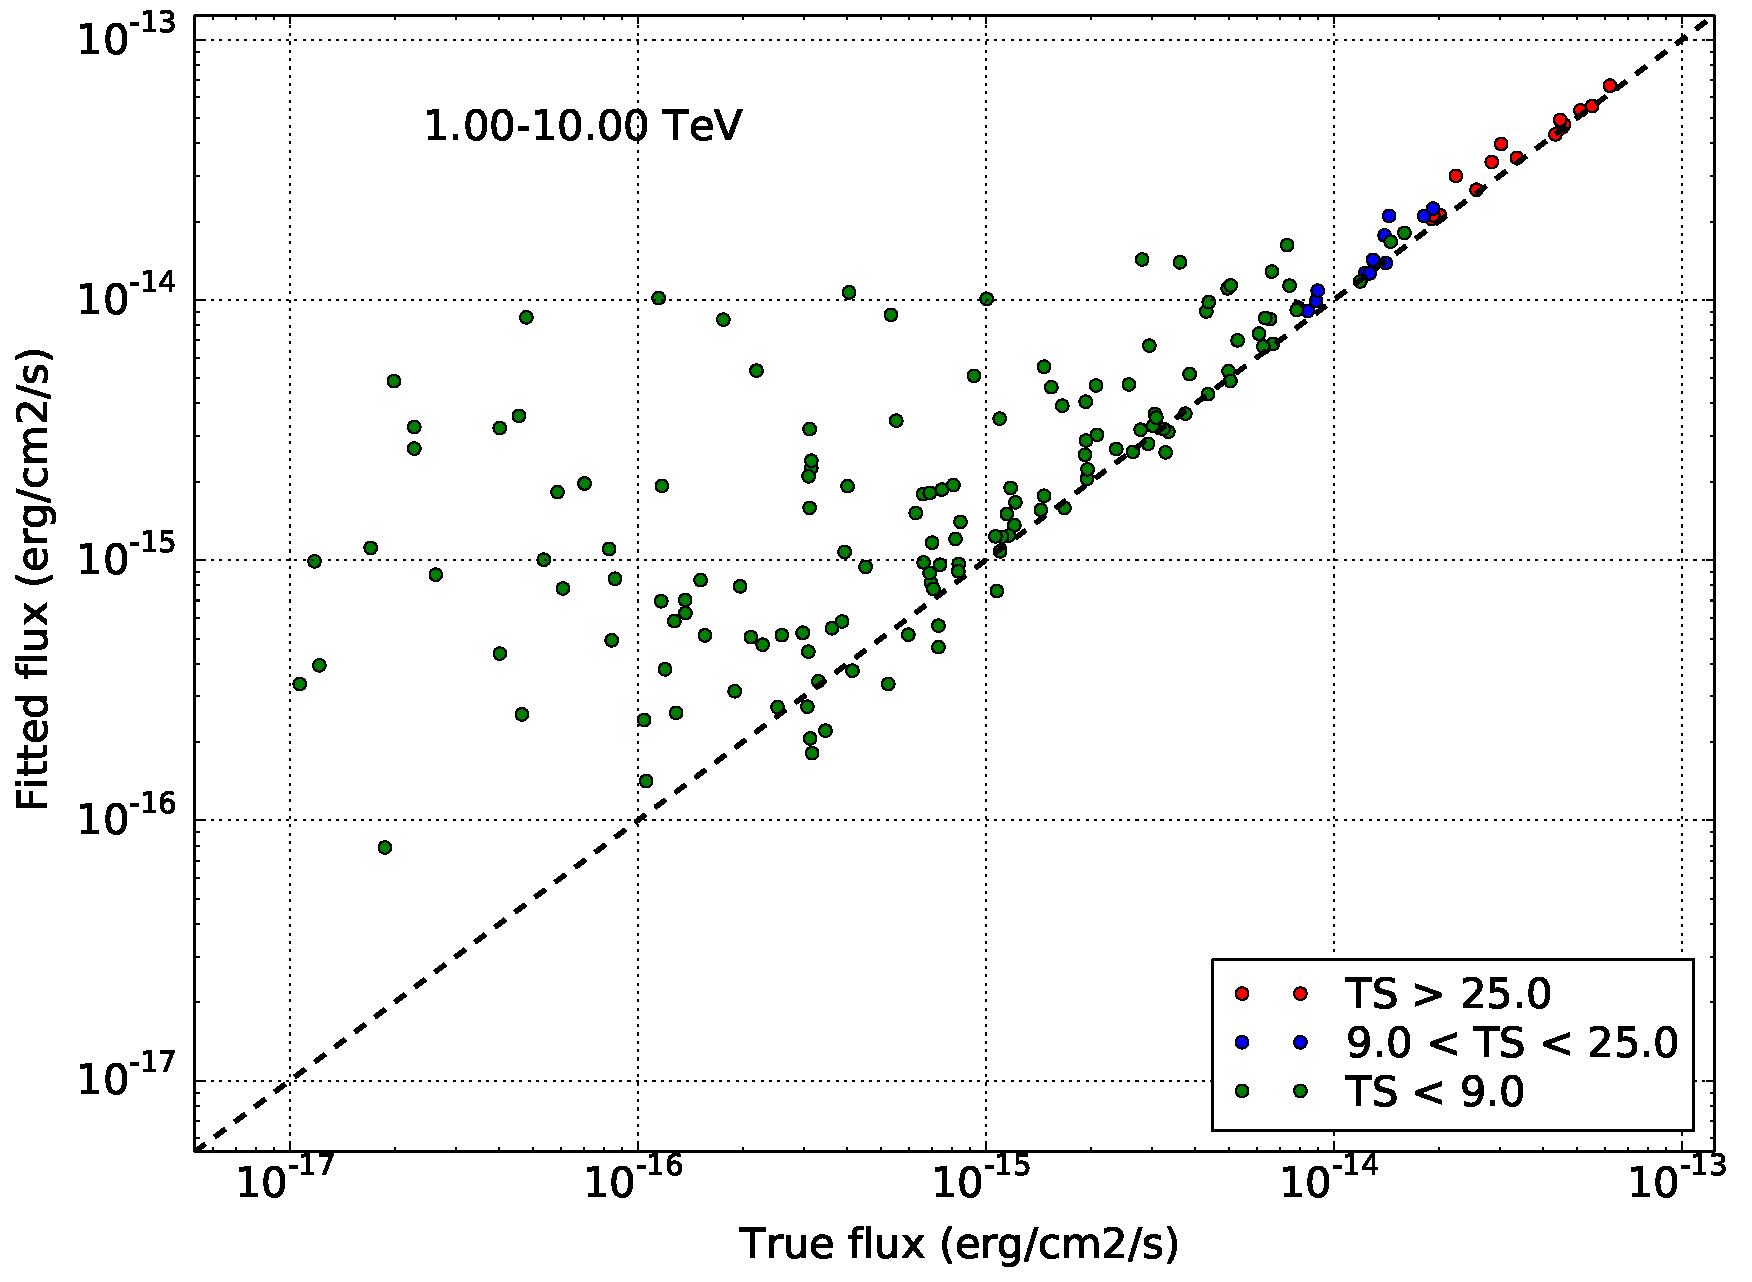
\includegraphics[width=1\textwidth]{Pictures/Flux_pop.pdf}
\endminipage 
\minipage{0.5\textwidth}
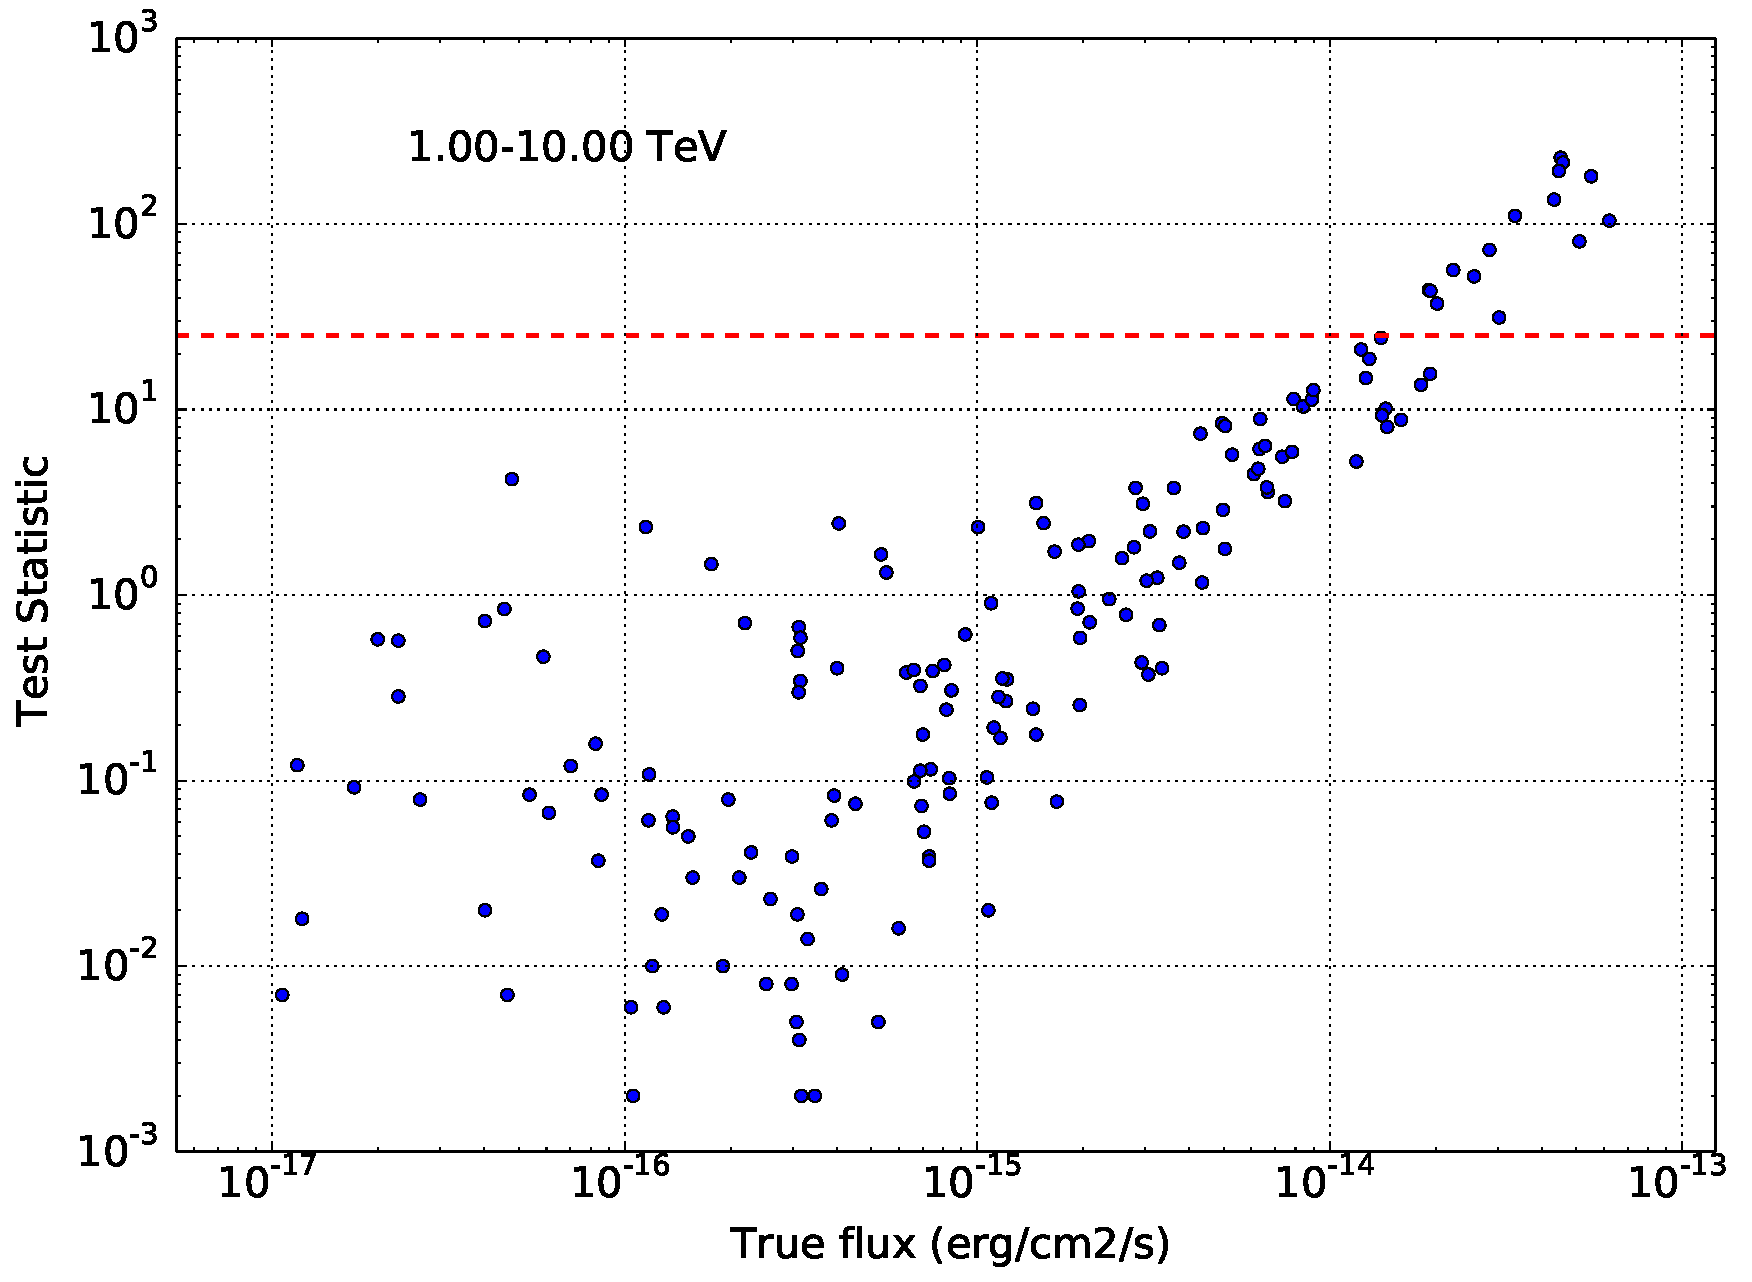
\includegraphics[width=1\textwidth]{Pictures/TS_pop.pdf}
\endminipage
  \caption{\textit{Left:} True flux vs. fitted flux for the synthetic population of \gls{pwne}. Each \gls{pwn} has been fitted individually, keeping the rest of the model components fixed. \textit{Right:} TS value vs. true flux of the \gls{pwne} population. Red line corresponds to TS=25 ($5\sigma$ detection significance).}
    \label{fig:pwnepopresults}
\end{figure}

\subsection{Diffuse Emission}

The diffuse emission models for pion-decay and \gls{ic} scattering have been fitted as mapcubes where the only free parameter left is the normalization. The fit in the full energy range has resulted in a positive detection for the pion-decay component, with a mean TS value of 29.06 (5.39$\sigma$ significance). For the \gls{ic} component, the TS obtained is 0.282, resulting in a non-detection. Upper limits for this model have been calculated instead, giving an upper limit at 99\% confidence level in the integral flux limit of $7.33\cdot10^{-12}$ ph cm$^{-2}$s$^{-1}$ in the range 100 GeV-100TeV. In figure \ref{fig:sensiulimits}, energy flux upper limits for three energy ranges (0.1-1 TeV, 1-10 TeV, 10-100 TeV) are shown.

\begin{figure}
  \centering
  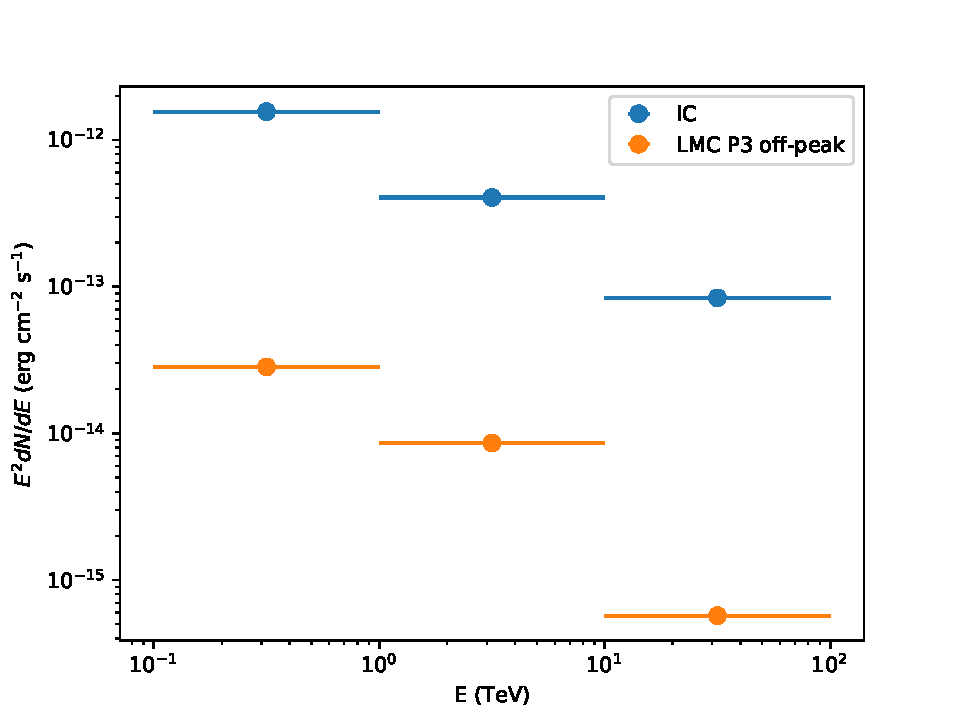
\includegraphics[width=0.7\textwidth]{Pictures/sensicurves_ic+lmcp3.pdf}
  \caption{\label{fig:sensiulimits} Energy flux upper limits computed for the \gls{ic} diffuse component and LMC P3 off-peak model in three energy ranges.}
\end{figure}
    
\section{Dark Matter annihilation in the LMC}\label{sec:dminlmc}

\par In this section, we will develop forecasts for the detection of an additional component of the diffuse gamma--ray sky due to an ``exotic''  source, namely the annihilation of \gls{dm}, under the assumption that the latter is made of stable particles which may however annihilate and produce a shower of standard model particles, which in turn would lead to either direct or secondary production of gamma--rays, at energies of GeVs and above, thus making them potentially detectable with \gls{cta} (and other gamma--ray telescopes).
We address the reader to the vast literature existing on the \gls{dm} candidates and models complying with the many requirements and characteristics (e.g. \cite{2010pdmo.book.....B, Boyarsky:2009ix, 2004NuPhB.683..219B, 2000PhRvL..85.1158H, Blais:2002nd} and references therein), adopting here the incorrect yet efficient (for our purposes here) definition of generic \glspl{wimp}.
The goal of this section is to explore whether \gls{cta} will be able to observe the annihilation of \glspl{wimp} in the \gls{lmc}, and if observations (or failure thereof) can be useful in the identification (or constrain) of \gls{dm} candidates. To this goal, it is useful to recall the fundamental equation relating the gamma--ray flux to the \gls{dm} quantities of interest:

\begin{equation}
    \frac{d \Phi}{dE}=\frac{1}{8 \pi} \frac{<\sigma v>}{m_{\chi}^2} \frac{d N_{\gamma}}{dE} \int_{\Delta\Omega}\int_{l.o.s} dl \rho^2(\vec{l})
\label{eq:dmflux}                                     
\end{equation}

 
where $\frac{d \Phi}{dE}$ is the gamma--ray flux contributing to the diffuse emission and potentially observable from the telescope, 
$\sigv$ is the \gls{dm} annihilation velocity-averaged cross section (in fact, a rate), $m_{\chi}$ is the mass of the \gls{dm} candidate, $\frac{dN_{\gamma}}{dE}$ is the gamma--ray spectrum produced by one single annihilation event (two \gls{dm} particle annihilating into a shower of  standard model particles), and $\rho(l)$ is the \gls{dm} density distribution within the target, with $l$ being a generic variable representing the line of sight.
We will accurately define the quantities of use in the rest of this Section, and otherwise follow standard convention (including units) as within the WIMP \gls{dm} community when non ambiguous, throughout our whole analysis.

It is important to stress that, according to the practise in the high energy \gls{dm} searches with gamma--rays, we will treat both $\sigv$ and $\mdm$ as free parameters, and adopt ``single annihilation'' spectra assuming at each time that the branching ratio of the reaction is one, namely that the entire annihilation happens in the specific channel, then showing the results for different channels in order to bracket the possible outcome. Model--specific analysis are outside the scope of this study.

 \subsection{LMC Dark Matter profile}
 \label{LMCprofile\gls{dm}}  
 \par The Dark Matter distribution of the \gls{lmc} can be inferred by the gravitational structure of its disk, following the well known ``rotation curve method''. This allows to infer the \gls{dm} component of the gravitational potential (often under an assumption of sphericity, which we will keep here) for disk galaxies in an extended mass range, once that a suitable set of tracers for the circular motion of the disk (at different galactocentric distances) and a good understanding of the visible component are available.
%  relying on the well-posed assumption (for disk and spiral galaxies in an extended mass range to which the LMC belongs to) that the stellar disk is in roto-gravitational equilibrium. 
In order to be consistent with previous literature and allow direct comparison, and at the same time perform independent analysis, we have followed closely the results of \cite{Buckley:2015doa}, which in turn adopts the data available in the literature and present in \cite{1998ApJ...503..674K,1992A&A...263...41L,vanderMarel:2013jza}.
We have adopted a Zhao six-parameters profile \cite{1996MNRAS.278..488Z}\footnote{When $\alpha$ = 1 and $\beta$ = 3 the Zhao profile is called generalised NFW profile (gNFW) with flexible inner \gls{dm} density slope $\gamma$.} (see Eq. \ref{gNFW}) 

\begin{equation}
    \rho(r) = \frac{\rho_{0}}{\left(\frac{r}{r_{S}}\right)^{\gamma}\left[ 1+\left(\frac{r}{r_{S}} \right)^{\alpha}\right]^{\frac{\beta-\gamma}{\alpha}}}
\label{gNFW}
\end{equation}

centered at  (RA: 80.0º,dec:-69.0), where $r_{S}$ is the scale radius and $\rho_{0}$ is the characteristic density. These two last parameters depend on the specific \gls{dm} halo. 
Setting $(\alpha,\beta,\gamma) = (1,3,1)$ we retrieve the \gls{nfw} profile \cite{NFW}. An isothermal profile is obtained setting $(\alpha,\beta,\gamma) = (2,2,0)$. Variations of these two profiles have been tested, with their parameters shown in table \ref{tab:dmprofiles} and plotted in figure \ref{fig:dmprofiles}. For the \gls{nfw} profile, a more cuspy profile with $\gamma=1.5$ and a more cored profile, with $\gamma=0.5$ are tested. In the case of the isothermal profile, the scale radius is varied from the iso-mean profile with $r_{S}$ = 2.4 (kpc) to iso-max with $r_{S}$ = 3 (kpc) and iso-min with $r_{S}$ = 1 (kpc).
We have performed sanity checks against the profiles adopted by \cite{Buckley:2015doa}. In particular, we have made sure that when using the same values of the \gls{dm} profile adopted by \cite{Buckley:2015doa}, we obtained compatible values for the convenient quantity often referred to as J--factor:
\begin{equation}
J(\Delta \Omega) \equiv \int_{\Delta\Omega}\int_{l.o.s} dl \rho^2(\vec{l})
\label{JfactorDef}
\end{equation}

\begin{figure}
        \centering  
        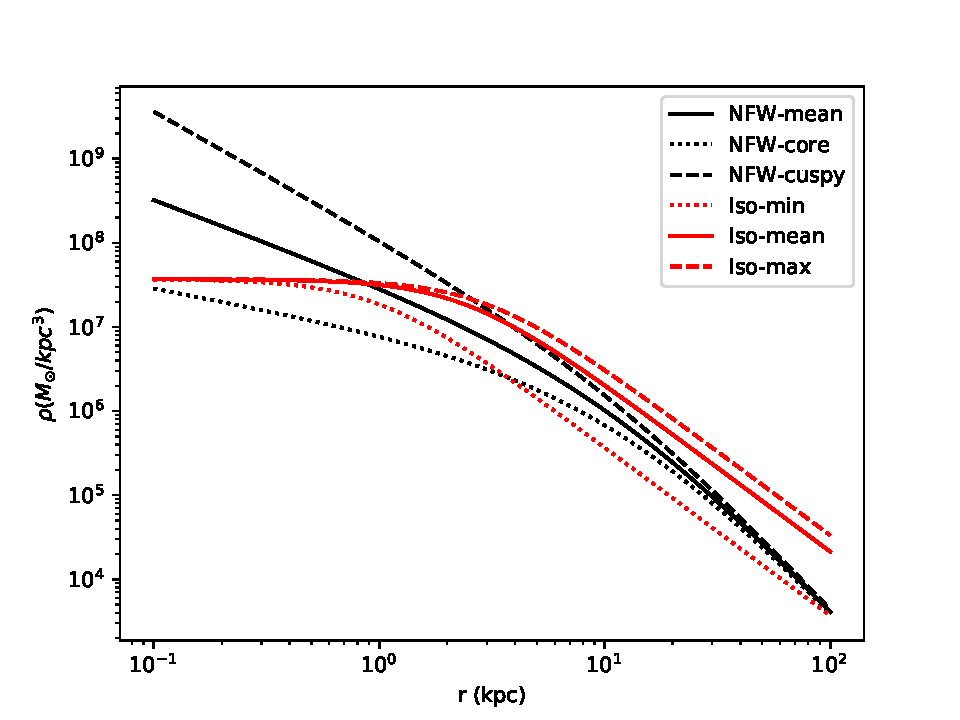
\includegraphics[scale=0.7]{Pictures/dmprofiles.pdf}
        \caption{\label{fig:dmdensity} \gls{dm} benchmark density profiles, computed using the parameters listed in table \ref{tab:dmprofiles}.} 
\end{figure}


May it be noticed that the steepness of the profile in the innermost regions is virtually unconstrained, thus allowing for the possibility of either shallow (cored) or steep (peaked) profiles without running into severe constraints from the kinematic data, as the central slope does not sensibly affect the gravitational structure of the galactic disk. At the same time, the steepness of the \gls{dm} profile has dramatic impact on the J--factor (as it can be appreciated from the square in Eq. \ref{JfactorDef}), thus affecting the final gamma--ray flux expected from the region. In order to bracket this uncertainty, we have chosen to adopt gNFW profile with different slopes, resembling

\par As of the actual implementation, we have used the public code {\tt CLUMPY}, a code for gamma--ray and neutrino signals from \gls{dm} structures \cite{2012CoPhC.183..656C, 2016CoPhC.200..336B, 2019CoPhC.235..336H}, to generate two-dimensional sky maps of the J-factor in Eq.~\eqref{JfactorDef}, with the parameters listed in table \ref{tab:dmprofiles}, in a field of view of 10$^{\circ}$. These sky maps correspond to the spatial part of the {\tt DiffuseMap} model (given in {\it ctools}) which are combined with the spectra of different annihilation channels in the final \gls{dm} emission model.

%\par We have taken $\gamma=1.0$ etc etc


\begin{table}
\centering
\addtolength{\tabcolsep}{6pt}
\renewcommand{\arraystretch}{1.1}
\scalebox{0.9}{%
\begin{tabular}{ | c | c | c | c | c | c | c |}
\hline
profile & $\alpha$ & $\beta$ & $\gamma$ & $r_s$ [kpc] & $\rho_0$ [$\rm M_{\odot}/kpc^3$] & $\mathcal{J}(10º)$ [$\rm GeV^2/cm^5$] \\
\hline \hline
{\tt iso-min} & 2 & 2 & 0 & 1 & $3.7\times10^7$ & $8.51\times 10^{19}$ \\
{\tt iso-mean} & 2 & 2 & 0 & 2.4 & $3.7\times10^7$ & $9.71\times 10^{20}$\\
{\tt iso-max} & 2 & 2 & 0 & 3 & $3.7\times10^7$ & $1.74\times 10^{21}$ \\
{\tt gnfw-core} & 1 & 3 & 0.5 & 12.6 & $2.6\times10^6$ & $5.13 \times 10^{20}$ \\
{\tt nfw-mean} & 1 & 3 & 1 & 12.6 & $2.6\times10^6$ & $1.36 \times 10^{21}$ \\
{\tt gnfw-cusp} & 1 & 3 & 1.5 & 12.6 & $2.6\times10^6$ & $4.22 \times 10^{22}$ \\
\hline
\end{tabular}}
\caption{Benchmark \gls{dm} profiles adopted in this work. The {\tt iso-mean} and {\tt nfw-mean} corresponds to the profiles from table II in \cite{Buckley:2015doa} with the same nomenclature. The $\mathcal{J}$ factor, in the last column, is integrated over a field of view of 10$^\rm o$.}
\label{tab:dmprofiles} 
\end{table}


 
 \subsection{Gamma Ray Spectrum}\label{\gls{dm}spectrumAnn}  
 
 For the spectral part of the \gls{dm} emission model ($dN_{\gamma}/dE$ in equation \ref{eq:dmflux}), the recipes from \cite{2011cirelli} were used, where the energy spectra of $\gamma$-rays produced by different \gls{dm} annihilation channels are provided. For this work, the studied channels were $b \overline b$, $W^+ W^-$, $\tau^+\tau^-$, $\mu^+ \mu^-$ including electro-weak corrections as computed in \cite{2011EWcorrections}, and their spectra can be seen in figure \ref{fig:dmspec}, computed for a set of \gls{dm} particle masses.

\begin{figure}
  \centering
  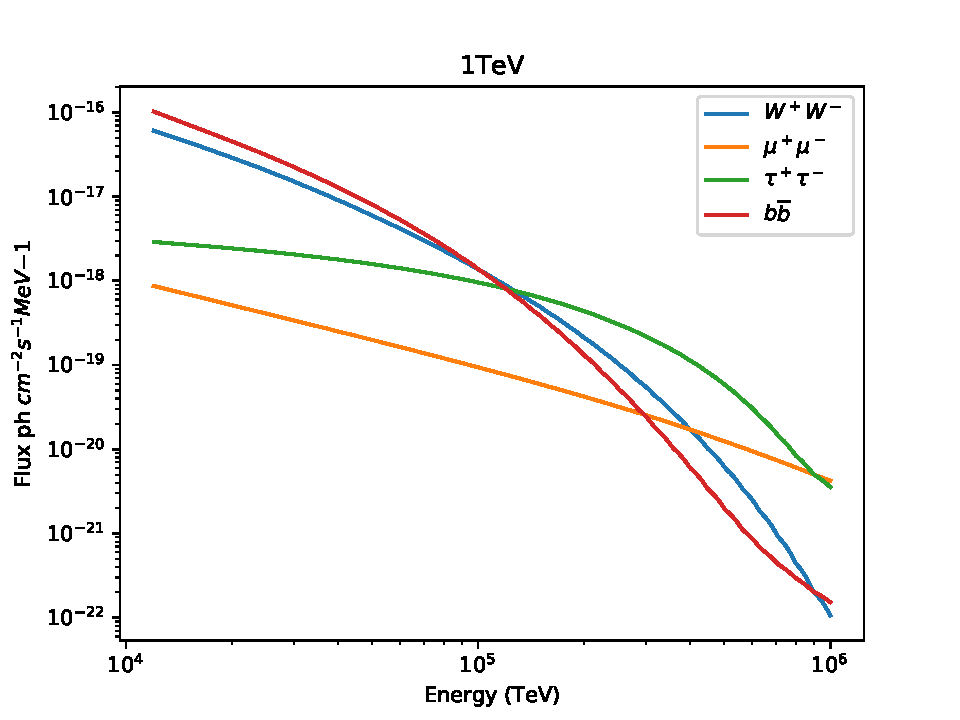
\includegraphics[width=0.6\textwidth]{Pictures/1tevspectra.pdf}
  \minipage{0.5\textwidth}
  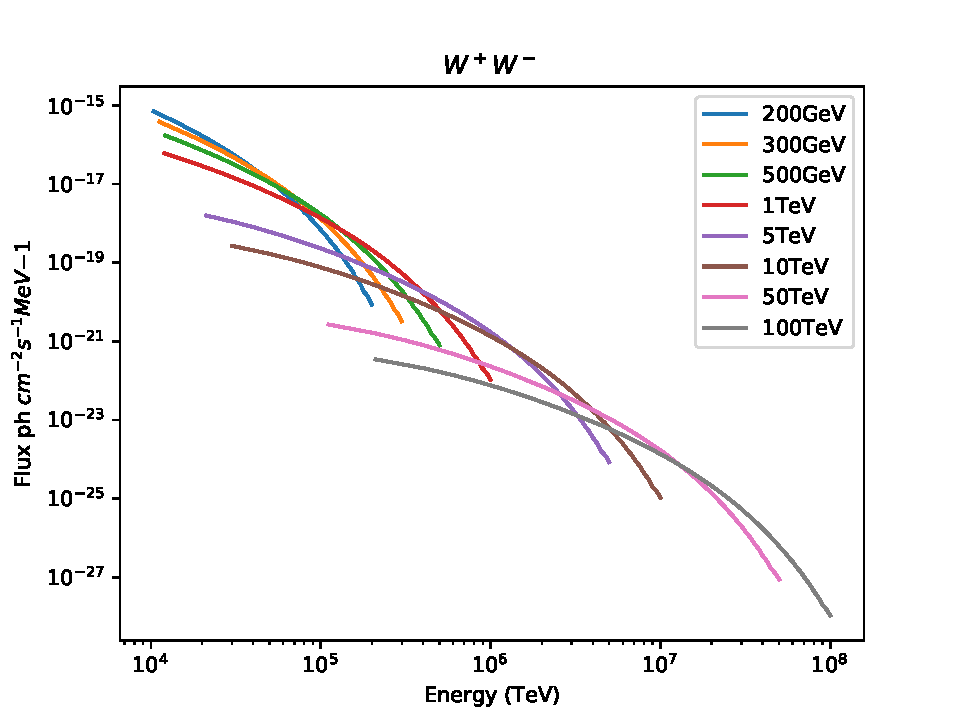
\includegraphics[width=1\textwidth]{Pictures/specW.pdf}
  \endminipage 
  \minipage{0.5\textwidth}
  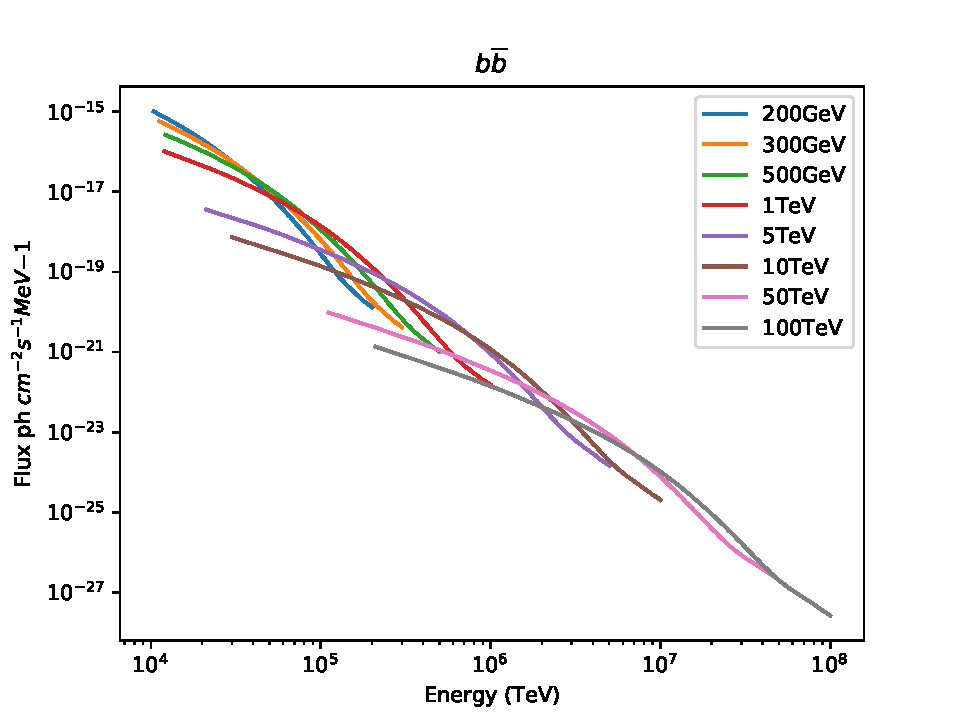
\includegraphics[width=1\textwidth]{Pictures/specb.pdf}
  \endminipage \\
  \minipage{0.5\textwidth}
  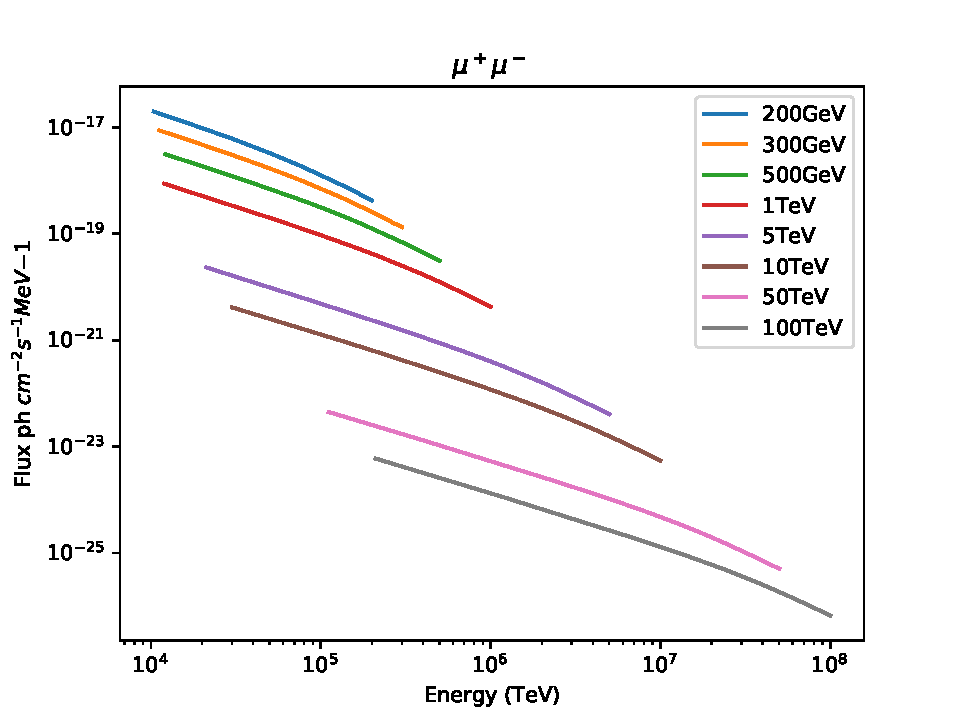
\includegraphics[width=1\textwidth]{Pictures/specMu.pdf}
  \endminipage
  \minipage{0.5\textwidth}
  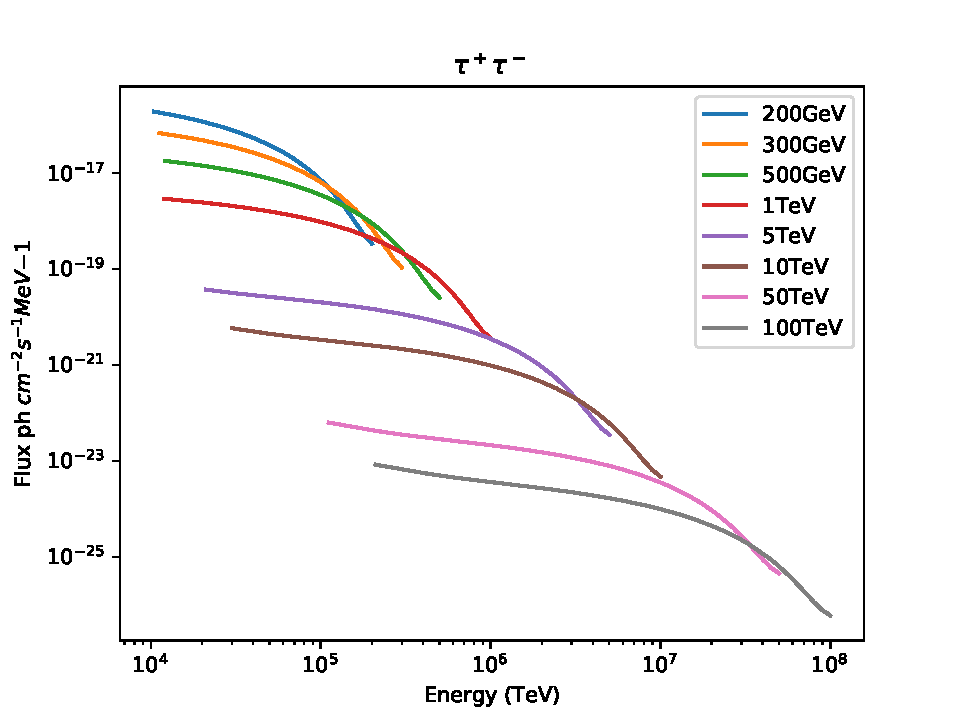
\includegraphics[width=1\textwidth]{Pictures/specTau.pdf}
  \endminipage \\
  \caption{$\gamma$-ray spectra of \gls{dm} pair annihilation, for different annihilation channels and masses of \gls{dm} particle. }
  \label{fig:dmspec}
\end{figure}
 
  \subsection{Dark Matter sensitivity curve}\label{LMCsenscurv\gls{dm}}

\par In line with the use of the literature, we do not attempt here at forecasts for a specific \gls{dm} candidate but rather at sampling the range of signal that should be expected within a ``standard'' \gls{wimp} scenario.
While treating $\sigv$ and $\mdm$ as independent variables, we sample the ``single particle'' spectrum of the annihilation, namely the gamma--ray produced in annihilation process which assumed the two \gls{dm} particles to annihilate in different types of standard model primaries, and generating a subsequent cascade of high energy photons. 

Using the \gls{dm} profiles and spectra described in previous section, a likelihood analysis was performed to obtain the minimum flux needed for the \gls{lmc} \gls{dm} component to be detectable by \gls{cta}. The asimov data set with the astrophysical $\gamma$-ray sources described in section \ref{sec:model} is used for this task as a background on top of which we calculate the flux needed to be emitted by each \gls{dm} model in order to be detected. To do so, the procedure for upper limits calculation described in section \ref{sec:ulimits} is applied. Each \gls{dm} model is included in the fitted model as a new source, for which the differential upper flux limit for a reference energy, the integrated upper flux limit over the energy range 0.1 GeV-\gls{dm} particle mass, and the integrated energy limit are calculated. In this analysis, the \gls{dm} particles mass and the velocity averaged annihilation cross section $\sigv$ are treated as independent variables. \\   
From the resulting flux  limit $\frac{d \Phi_{ulim}}{dE}$, from equation \ref{eq:dmflux}, the limit on $\sigv$ can be extracted. The sensitivity curves where $<\sigma v>$ is plotted versus \gls{dm} particle masses are shown in figure \ref{fig:dmsensicurves}. Each curve corresponds to a specific \gls{dm} profile and annihilation channel. The space above the curves represent the parameter space of $<\sigma v>$ and \gls{dm} mass that could be explored by \gls{cta}.

\begin{figure}
\centering
\minipage{0.5\textwidth}
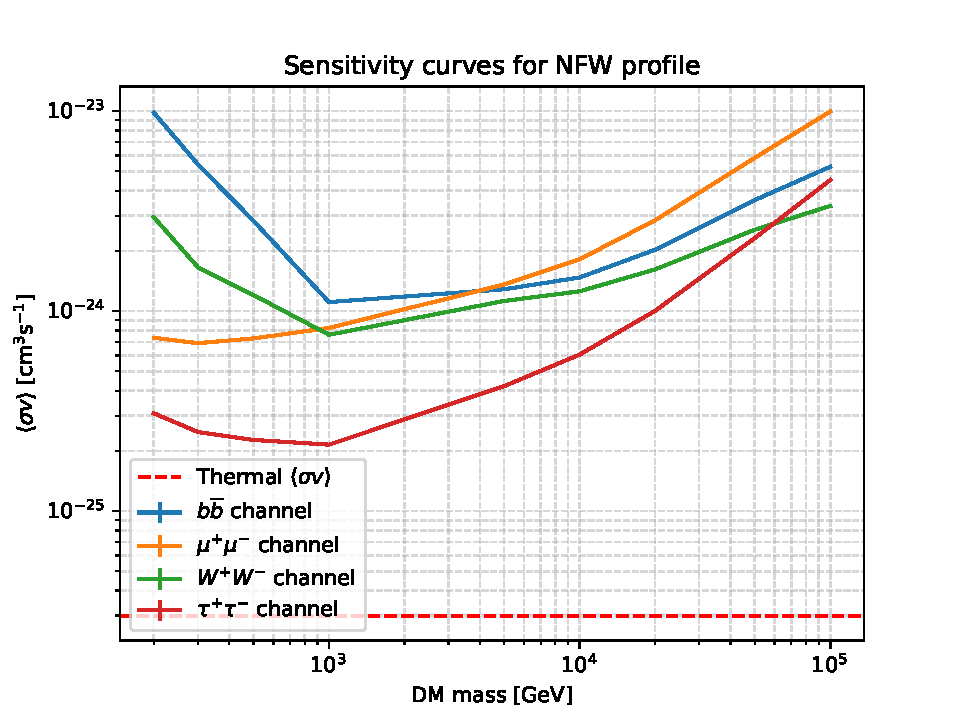
\includegraphics[width=1\textwidth]{Pictures/Limits_NFW.pdf}
\endminipage 
\minipage{0.5\textwidth}
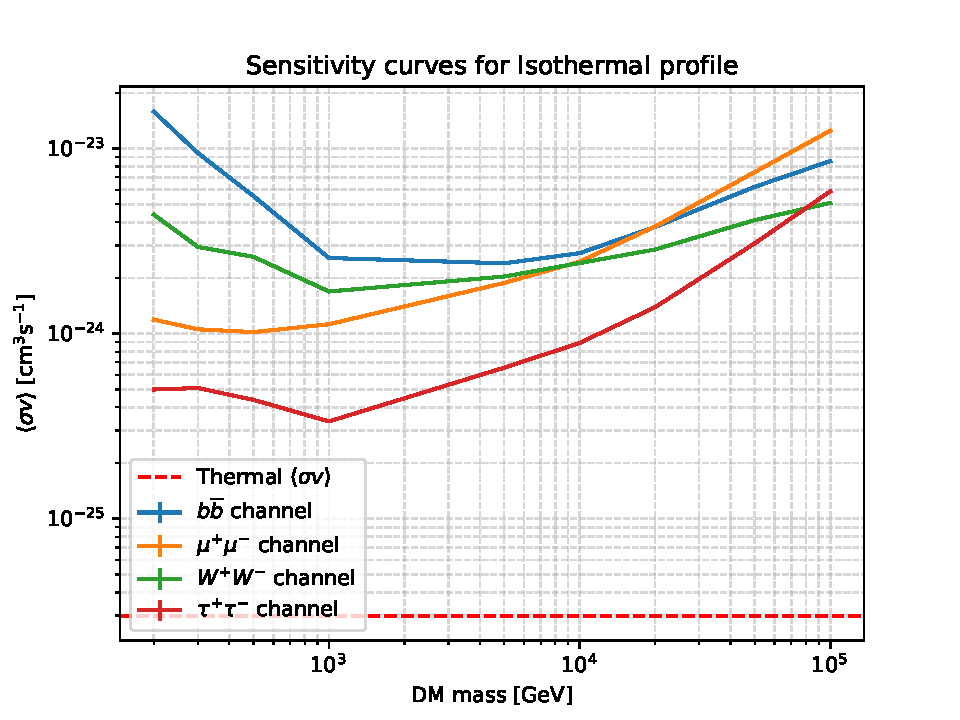
\includegraphics[width=1\textwidth]{Pictures/Limits_Isothermal.pdf}
\endminipage \\
\minipage{0.5\textwidth}
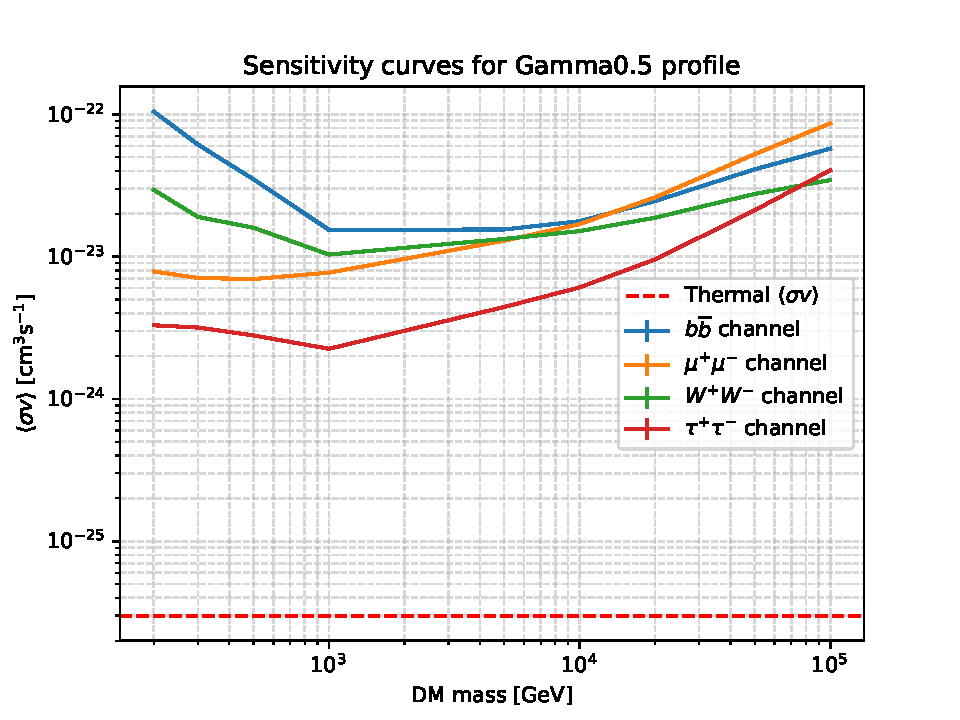
\includegraphics[width=1\textwidth]{Pictures/Limits_Gamma0-5.pdf}
\endminipage
\minipage{0.5\textwidth}
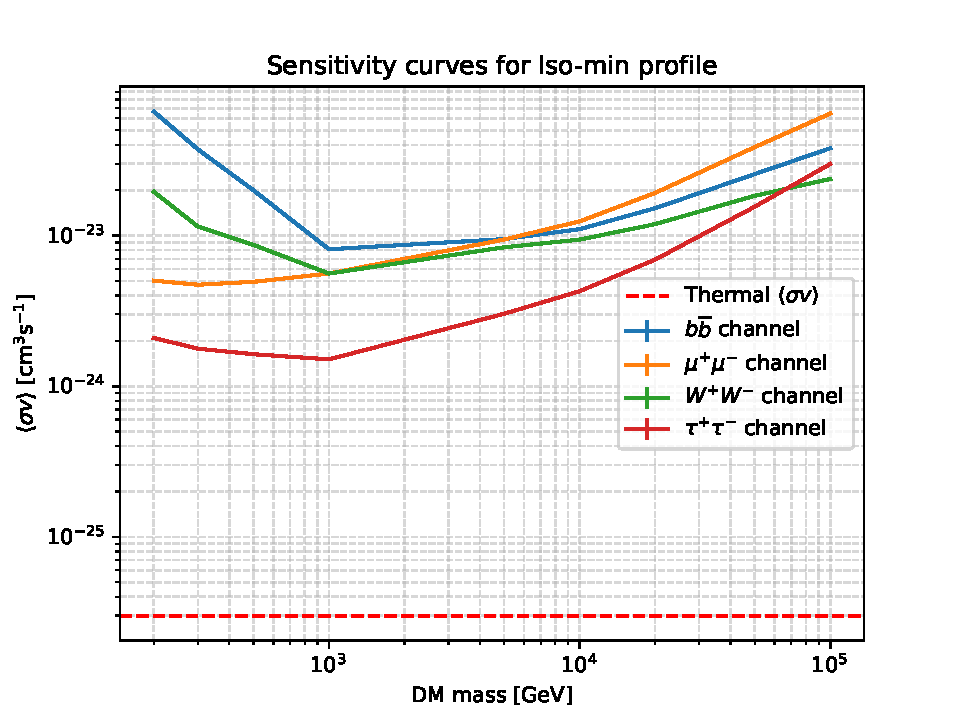
\includegraphics[width=1\textwidth]{Pictures/Limits_Iso-min.pdf}
\endminipage \\
\minipage{0.5\textwidth}
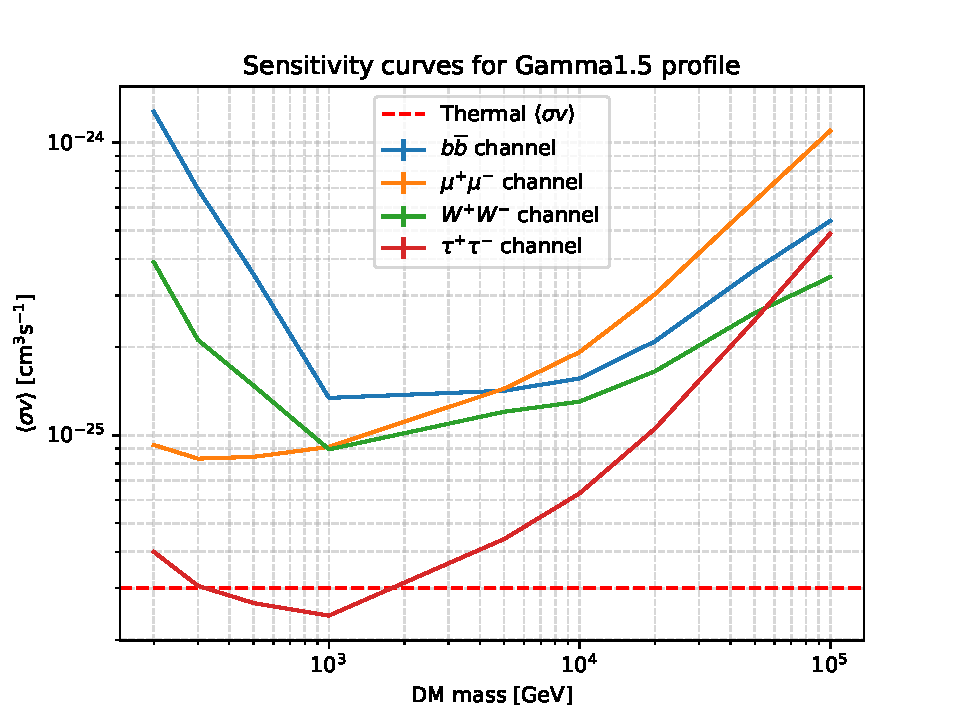
\includegraphics[width=1\textwidth]{Pictures/Limits_Gamma1-5.pdf}
\endminipage
\minipage{0.5\textwidth}
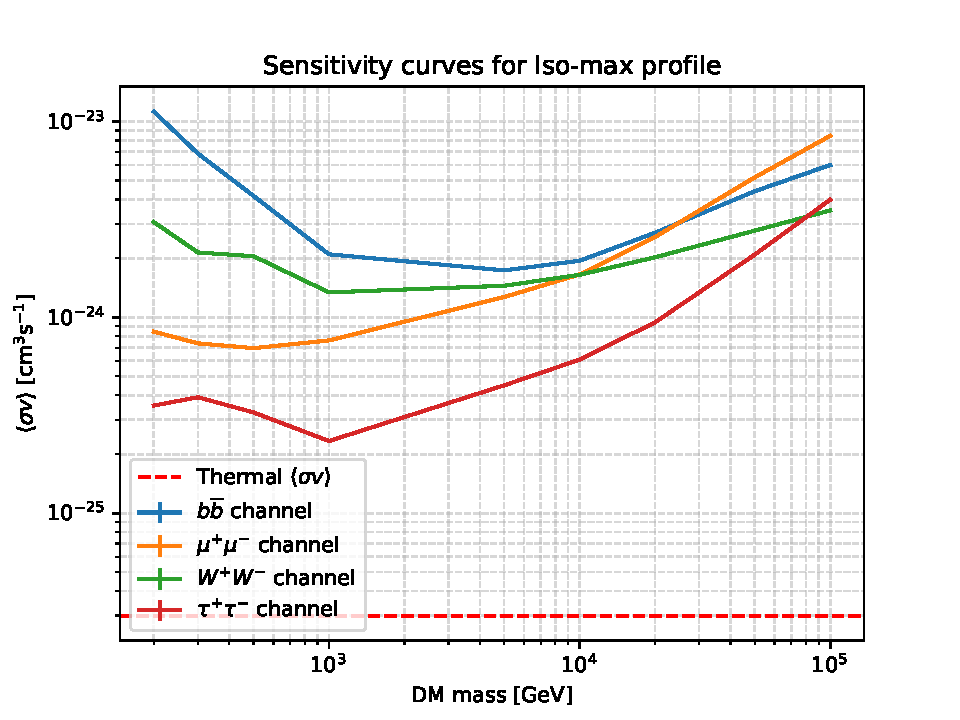
\includegraphics[width=1\textwidth]{Pictures/Limits_Iso-max.pdf}
\endminipage
  \caption{Sensitivity curves of $<\sigma v >$ vs. \gls{dm} particle mass, resulting for the profiles listed in table \ref{tab:dmprofiles}, and for four annihilation channels: $b\overline b$, $W^+W^-$, $\mu^+ \mu^-$, $\tau^+ \tau^-$.}
    \label{fig:dmsensicurves}
\end{figure}

\section{Systematics} \label{sec:systematics}
Whatever we want to say about systematics.
\section{Summary and Conclusions} \label{sec:conclusions}

The deep survey of the \gls{lmc} will be an ambitious task which will account for many challenges, but that will potentially provide many scientific results and new discoveries. Besides a lot of work can be done in the subjects until \gls{cta} is fully available, in this work the first hints on the possible results of the survey have been studied.\\
Regarding the known point sources observed by other $\gamma$-ray experiments, a remarkable high significance has been obtained for all of them, meaning they will be easily detected within the survey with a binned likelihood analysis, which will allow to characterize the sources spectra in the \gls{cta} range, at least over 100 GeV. Given the duration of the survey (>300 h), it will also be possible to study the variability of LMC-P3, for which an upper flux limit for the off-peak emission has been derived. From the artificial population of \gls{pwne} introduced in the emission model, for 15 a significance sufficiently large to be detected has been obtained, providing an estimation of the number of new sources of this kind that \gls{cta} will be able to detect. The computed distribution of \gls{pwne} will serve as a trace for the blind search when dealing with real data from the survey.\\
One of the most interesting features of the \gls{lmc} is the fact that, as an extended source, it is possible to study the structure of its $\gamma$-ray emission, allowing to probe models of \gls{cr} injection and propagation. In this work, two models of diffuse emission of \gls{cr} due to leptonic \gls{ic} scattering and hadronic interactions leading to pion decay have been tested. The possibility to take into account the structure and distribution of \gls{cr} sources in the \gls{lmc} leads to the positive result on the detection of pion-decay emission following the model described in section \ref{sec:diffusemodel}. This is however a best-case scenario, where uncertainties in the model are not taken into account. However, it is an encouraging result to make efforts on the refinement of the analysis and model computation of the diffuse emission in the \gls{lmc} for the future real data. The \gls{ic} component, on the other hand, has resulted in a too low significance, meaning it would be not possible to disentangle this emission component from the rest of the background. An upper flux limit has been derived instead for this model.\\

Finally, prospects on the detection of a possible $\gamma$-ray signal from \gls{dm} annihilation have been calculated. The results have established the parameter space of \gls{dm} models which will be possible to study with \gls{cta}. The main reasons to point towards the \gls{lmc} were its extended nature, which allow to rely on \gls{dm} spatial structure for its differentiation from the background and its relatively high J-factor, comparable to other popular \gls{dm} candidates such as \gls{dsphe}. However, the big population of other $\gamma$-ray emitters difficult the task of extracting a $\gamma$-ray signal coming from \gls{dm} annihilation. In the results presented in this work, several \gls{dm} profiles, annihilation channels and \gls{dm} particle masses has been tested on top of the emission model of the \gls{lmc} to compute the velocity averaged annihilation cross section needed for the model to be detected. It can be seen from picture \ref{fig:dmsensicurves}, that the majority of the models lie several orders of magnitude over the canonical thermal cross section, which is the self-annihilation cross section of \gls{wimp} \gls{dm} in the case of being a thermal relic. This result predicts that \gls{cta} will unlikely be able to exclude the canonical cross section for the typical \gls{wimp} \gls{dm} models, except for the most cuspy ones(yet not very realistic) at \gls{dm} masses $\sim 1 TeV$ (case of nfw-cuspy profile and $\tau^+ \tau^-$ channel).\\

The work performed within the scope of this article will serve as a starting point for the future work that can be done regarding the \gls{lmc} \gls{ksp}. The emission model developed to perform the predictions presented will serve as a benchmark for future studies and for the analysis of real data from the \gls{lmc} survey.
Other topics which have been left out of the scope of this work, but which still will benefit from its results could be: A more detailed and realistic study on the possible new discovered sources, performing a totally blind search over the \gls{pwne} population, study a population of \glspl{snr}, or focus on other specific known sources not yet detected in the \gls{vhe} range, such as \gls{snr} 1987A.

\printbibliography
\end{document}
 
 

